%%%%%%%% ICML 2021 EXAMPLE LATEX SUBMISSION FILE %%%%%%%%%%%%%%%%%

\documentclass{article}

% Recommended, but optional, packages for figures and better typesetting:
\usepackage{microtype}
\usepackage{graphicx}
\usepackage{subfigure}
\usepackage{booktabs} % for professional tables
\usepackage{amsthm,amsmath,amsfonts,amssymb,bbm}

\newtheorem{axiom}{Axiom}
\newtheorem{claim}[axiom]{Claim}
\newtheorem{theorem}{Theorem}[section]
\newtheorem{lemma}[theorem]{Lemma}
\newtheorem{assumption}[theorem]{Assumption}
%%%%%%%%%%%%%%%%%%%%%%%%%%%%%%%%%%%%%%%%%%%%%%
%\theoremstyle{plain}
%\theoremstyle{remark}
\theoremstyle{remark}
\newtheorem{definition}[theorem]{Definition}
\newtheorem*{remark}{Remark}
\newtheorem{example}{Example}
\newtheorem*{fact}{Fact}
% hyperref makes hyperlinks in the resulting PDF.
% If your build breaks (sometimes temporarily if a hyperlink spans a page)
% please comment out the following usepackage line and replace
% \usepackage{icml2021} with \usepackage[nohyperref]{icml2021} above.
\usepackage{hyperref}

% Attempt to make hyperref and algorithmic work together better:
\newcommand{\theHalgorithm}{\arabic{algorithm}}

% Use the following line for the initial blind version submitted for review:
\usepackage{icml2021}

% If accepted, instead use the following line for the camera-ready submission:
%\usepackage[accepted]{icml2021}

% The \icmltitle you define below is probably too long as a header.
% Therefore, a short form for the running title is supplied here:
\icmltitlerunning{Submission and Formatting Instructions for ICML 2021}

\begin{document}

\twocolumn[
\icmltitle{Manifold Fitting and Projection via Quadratic Approximation}

% It is OKAY to include author information, even for blind
% submissions: the style file will automatically remove it for you
% unless you've provided the [accepted] option to the icml2021
% package.

% List of affiliations: The first argument should be a (short)
% identifier you will use later to specify author affiliations
% Academic affiliations should list Department, University, City, Region, Country
% Industry affiliations should list Company, City, Region, Country

% You can specify symbols, otherwise they are numbered in order.
% Ideally, you should not use this facility. Affiliations will be numbered
% in order of appearance and this is the preferred way.
\icmlsetsymbol{equal}{*}

\begin{icmlauthorlist}
\icmlauthor{Aeiau Zzzz}{equal,to}
\icmlauthor{Bauiu C.~Yyyy}{equal,to,goo}
\icmlauthor{Cieua Vvvvv}{goo}
\icmlauthor{Iaesut Saoeu}{ed}
\icmlauthor{Fiuea Rrrr}{to}
\icmlauthor{Tateu H.~Yasehe}{ed,to,goo}
\icmlauthor{Aaoeu Iasoh}{goo}
\icmlauthor{Buiui Eueu}{ed}
\icmlauthor{Aeuia Zzzz}{ed}
\icmlauthor{Bieea C.~Yyyy}{to,goo}
\icmlauthor{Teoau Xxxx}{ed}
\icmlauthor{Eee Pppp}{ed}
\end{icmlauthorlist}

\icmlaffiliation{to}{Department of Computation, University of Torontoland, Torontoland, Canada}
\icmlaffiliation{goo}{Googol ShallowMind, New London, Michigan, USA}
\icmlaffiliation{ed}{School of Computation, University of Edenborrow, Edenborrow, United Kingdom}

\icmlcorrespondingauthor{Cieua Vvvvv}{c.vvvvv@googol.com}
\icmlcorrespondingauthor{Eee Pppp}{ep@eden.co.uk}

% You may provide any keywords that you
% find helpful for describing your paper; these are used to populate
% the "keywords" metadata in the PDF but will not be shown in the document
\icmlkeywords{Machine Learning, ICML}

\vskip 0.3in
]

% this must go after the closing bracket ] following \twocolumn[ ...

% This command actually creates the footnote in the first column
% listing the affiliations and the copyright notice.
% The command takes one argument, which is text to display at the start of the footnote.
% The \icmlEqualContribution command is standard text for equal contribution.
% Remove it (just {}) if you do not need this facility.

%\printAffiliationsAndNotice{}  % leave blank if no need to mention equal contribution
\printAffiliationsAndNotice{\icmlEqualContribution} % otherwise use the standard text.

\begin{abstract}

Manifold fitting is an emerging filed with an interaction of statistics and geometry. In this paper, we propose to fit the manifold with a quadratic function defined on the tangent space with a specific form. Compared with the existing linear-approximation methods, the quadratic-approximation approach can fit the unknown manifold with higher precision. Because a more complicated function is adopted in our manifold fitting process, the pulling-back approach turns the linear least-squares problem into a nonlinear quartic minimization problem. By bringing in the auxiliary function, we solve the quartic by repeatedly solving a series of quadratic minimization problems. Numerical experiments demonstrate that our method has a strong recovery capability compared with other current methods.

%This document provides a basic paper template and submission guidelines.
%Abstracts must be a single paragraph, ideally between 4--6 sentences long.
%Gross violations will trigger corrections at the camera-ready phase.
\end{abstract}

\section{Introduction}

The data residing in the high-dimensional ambient space often have some low-dimensional structure, because of the principal factors which affect the intrinsic generation process are often very limited. The locations of earthquakes or volcanos which caused by the crustal movement can be thought as the points residing on the one-dimensional manifold or the principal flow \cite{panaretos2014principal,davenport2010joint}.

In deep learning approach \cite{NIPS2014_5ca3e9b1}, using a network with fine-tuning parameters, we can transfer a very low-dimensional data into a very complicated image which some specific meaning. Also, we can use a simple sentence to generate a vivid picture  by a well-trained network. These phenomena indicate that very huge amount of data in our daily life are low-dimensional.

 
To handle the high-dimensional data, there are mainly two approaches. First, reconstruct the data in the low-dimensional space, such that, the reconstructed data in the low-dimensional space also keeps the relation (such as distance, geometry, affine transformation etc) in high dimensional space. This approach containing lots of classical dimension reduction works, such as LLE \cite{roweis2000nonlinear}, LTSA \cite{zhang2004principal}, Isomap \cite{tenenbaum2000global}, Eigenmap \cite{belkin2003laplacian}.
 
 The other approach try to fit a new smooth manifold by reducing the noise existing in the data. After the fitting process, the true signal will be strengthened and the noise factors will be diminished. Kernel density estimation \cite{genovese2014nonparametric,ozertem2011locally} is a very popular tool for the manifold fitting by transforming the manifold fitting problem into the ridge estimation problem. The ridge is defined as the set of points which satisfy some relation on gradient and Hessian of the density function. Overall, all the manifold fitting process can be considered with two steps. First, estimate the tangent space which is often implemented through the eigenvalue-decomposition of the covariance matrix. Second,  estimate an attraction force which is a  direction which points to somewhere near the manifold, this direction often constructed via the weighted shift-mean approach. By using the subspace constraint mean shift algorithm, we can move the outlier onto the manifold to some degree.
 
% The approximation error for the local affine space will yield an approximate error of $\|\tau\|_2^2$, where $\tau$ is the local coordinate. In other words, when we restrict the error subjects to the condition $\|\tau\|_2^2\leq \epsilon$, the maximum radius of the valid region is with the order of $\epsilon^{1/2}$. In this paper, we propose to approximate the manifold via the quadric function, by adopting this strategy, the approximation error will become $\|\tau\|_2^3$.  With the same precision requirement $\epsilon$, we have the maximum radius of our interested region is of the order $\epsilon^{1/3}$. Normally, $\epsilon$ is some scalar less than $1$, in this way, the quadratic approximation is a better approximation compared with the tangent affine plane.That is to say, to achieve the same precision, we will need much less times of fitting process.

A good approximation of the underlying manifold is the first step in our manifold fitting problem. The second important step needs to project the noisy data onto the fitted manifold which we obtained in the first step. Here, the term `project' has two meanings. First, the distance should be minimum, second, the direction of the projection should be perpendicular with the tangent place of the fitted manifold. A major reason for the linear approximation to be very widely used is the form of projection yields a quite simple linear least square problem.


%\begin{figure}[h] %  figure placement: here, top, bottom, or page
%   \centering
%   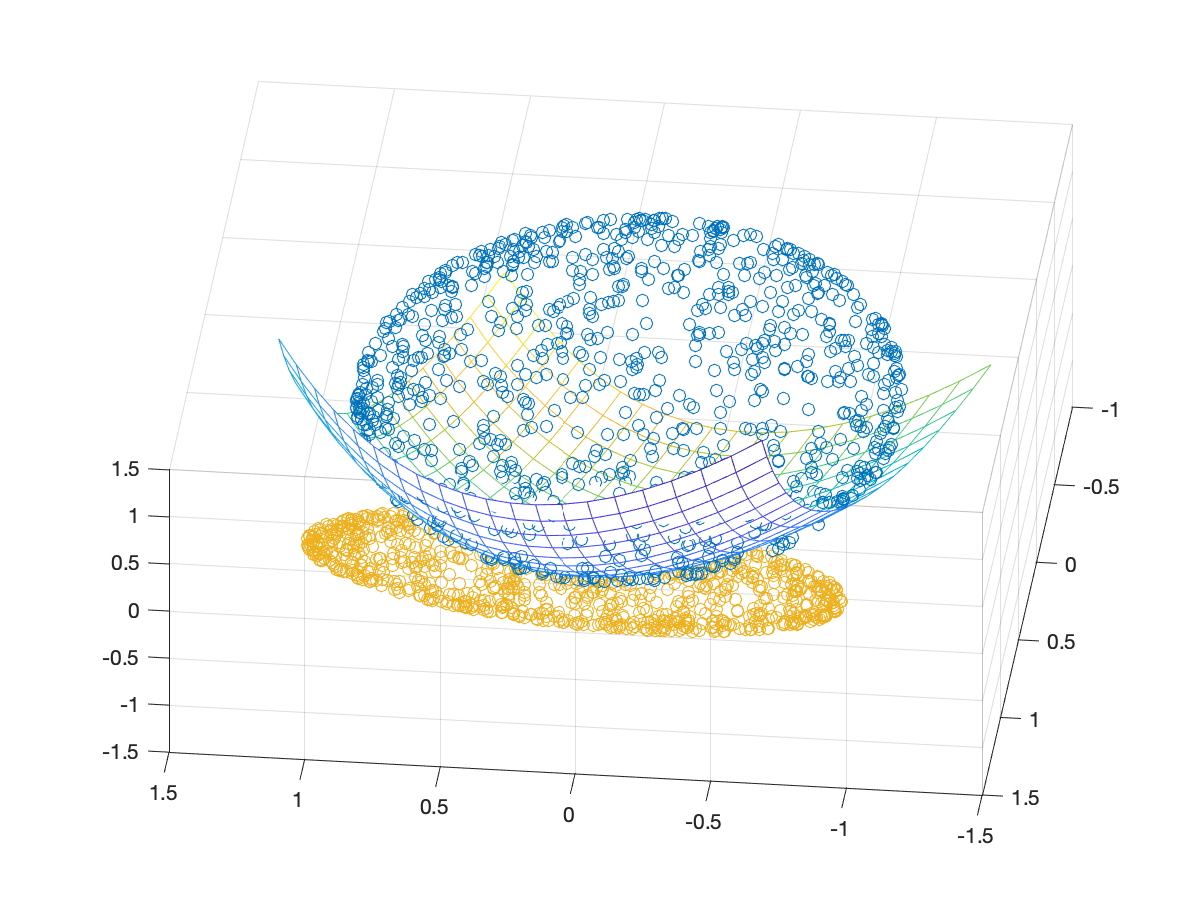
\includegraphics[width=3in]{demo.eps} 
%   \caption{ Fitting a manifold with the elliptical paraboloid surface}
%   \label{3-D paraboloid}
%\end{figure}

\subsection{Model Setting}
In this paper, we are not concentrating on finding the representation of $\phi(\tau)$ under the noiseless assumption. Instead, we assume to have the observations drawn from some low-dimensional manifold and disturbed by some noise, i.e, 
\[
x_i = \tilde{x}_i+\epsilon_i, \quad \tilde{x}_i \in \cal M,
\]
where $\epsilon_i$ is the noise which obeys some distribution, such as the multi-dimensional gaussian distribution.
Since the observations $\{x_i, i=1:n\}$ are discrete distributed, the idea of manifold fitting aims at generalizing the discrete data and obtaining a lower-dimensional approximation of the dataset. The manifold fitting approach can be written as a parametric estimation problem under the observations and the constrained model $\cal G$, i.e,
\begin{equation}\label{estimator1}
 \theta_* =\arg \min_\theta  \sum_i {\rm Loss}(x_i, {\cal G}, \theta ),
\end{equation}
where $\cal G$ represents the abstract model and $\theta$ represents the parameters within the model $\cal G$. Different models (such as linear or nonlinear) correspond to different $\cal G$. When we obtain our best parameter $\theta_*$ from \eqref{estimator1}, we can use the model ${\cal G}(\theta_*)$ to refine the outlier $x$ using the projection $P_{{\cal G}(\theta_*) }(x)$ via solving the following minimization problem:
\[
P_{{\cal G}(\theta_*) }(x) = \arg \min_{y\in {\cal G}(\theta_*) } \|x-y\|_2.
\]
 
The works such as \cite{genovese2014nonparametric,ozertem2011locally} all focus on how to get a better affine space to locally approximate the distribution of the data, i.e, in their works, ${\cal G}(\theta)$ is a linear model. However, at far as we know, the result of linear approximation approach relies heavily on the selection of the origin point (the red dot in Figure \ref{Comparison} ). An origin selected with good quality will surly improve the ability of recovery of the projection. However, in most of the cases, the origin can only be selected approximately as the underlying manifold is unknown.

\subsection{Manifold Parameterization}
For any manifold $\cal M$ and any point $x_0\in \cal M$, there is a corresponding twice differentiable function $\phi_{x_0}(\tau)$ 
%\begin{figure}[h!] %  figure placement: here, top, bottom, or page
%   \centering
%   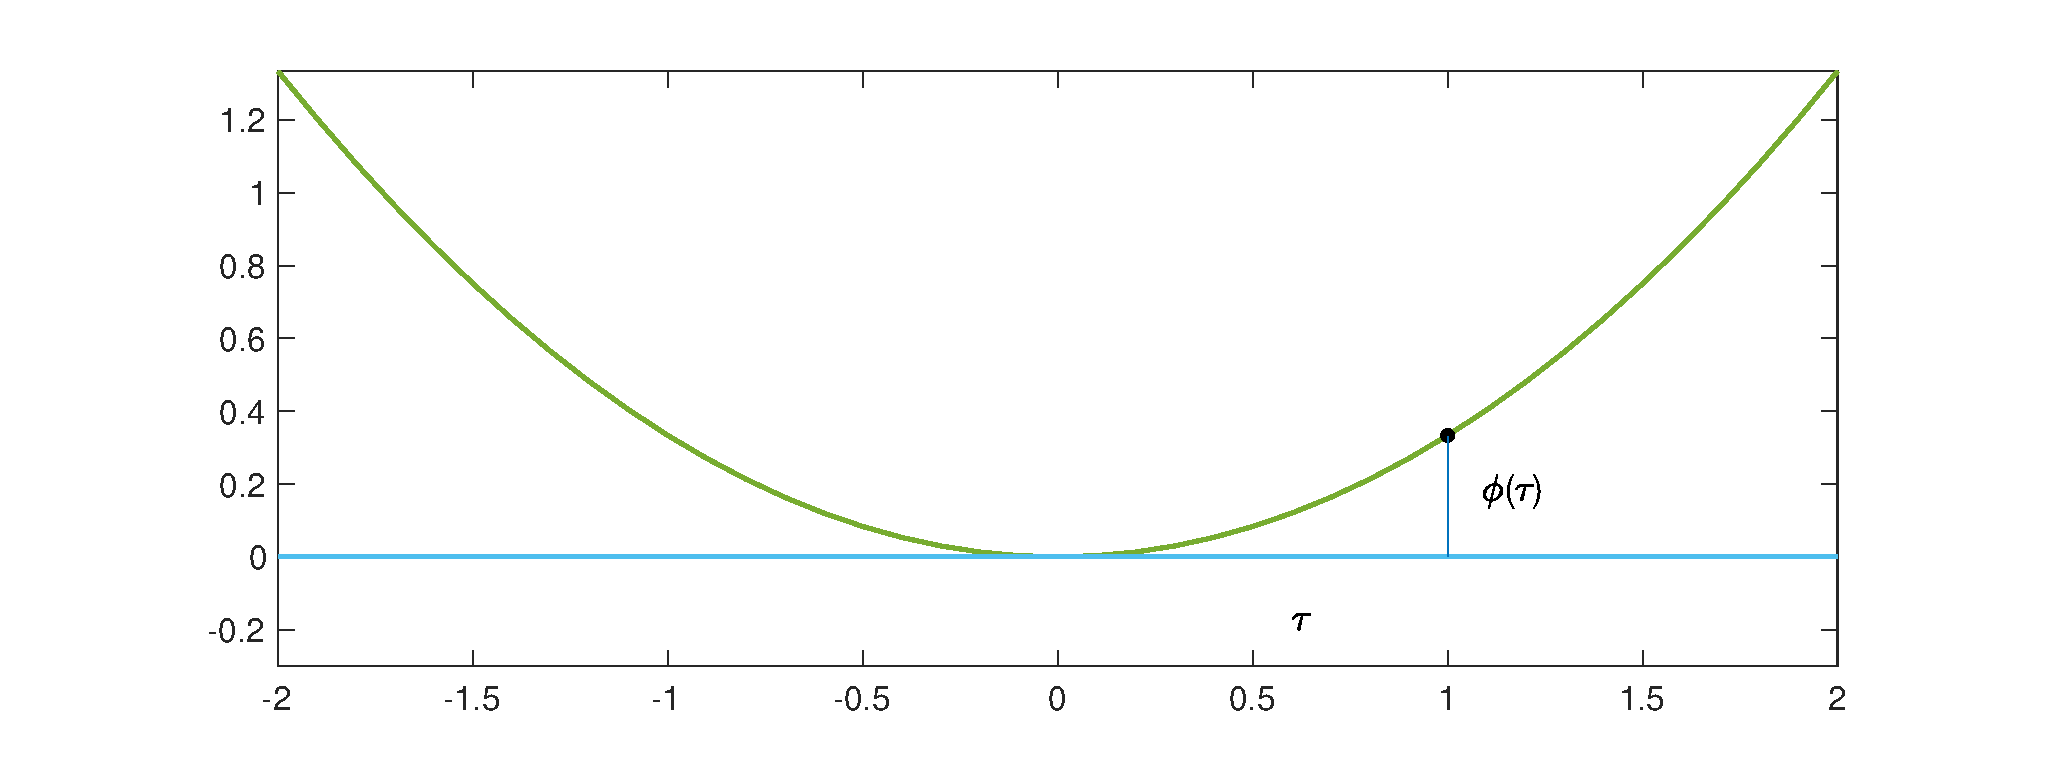
\includegraphics[width=\linewidth]{demo_phi.eps} 
%   \caption{Geometric interpretation of $\tau$ and $\phi(\tau)$ for a  1-D manifold embedded in 2-D}
%   \label{3-D paraboloid}
%\end{figure}
\[
\phi_{x_0}(\tau):{\mathbb R}^d\rightarrow {\mathbb R}^{D-d},
\]
such that every point within a local domain ${\cal D}_{x_0}(r)$ of $\cal M$, can be written with a parameterization form of 
\begin{equation}\label{manifold}
x(\tau)=  x_0 + U_{x_0} \tau+ U_{x_0}^{\perp} \phi_{x_0} (\tau),
\end{equation}
where the columns of $U_{x_0}$ are the basis on the tangent space and the columns in $U_{x_0}^{\perp}$ are the basis on the normal space. 

%
%In other words, corresponding to $x_0$ and $\cal M$, there is some radius $r$, such that:
%\begin{equation}\label{model}
% {\cal M}\cap {\cal D}_{x_0}(r) =  \{y | y =  x_0 + U_{x_0} \tau+ U_{x_0}^{\perp} \phi_{x_0} (\tau), \tau\in {\mathbb R}^d\}\cap {\cal D}_{x_0}(r).
%\end{equation}
%where ${\cal D}_{x_0}(r) = \{x|\|x-x_0\|\leq r\}$, $\phi_{x_0}(\tau)=[\phi_{x_0}^{d+1}(\tau),...,\phi_{x_0}^{D}(\tau)]^T$  is the function defined on the tangent space, the range of $\phi_{x_0}(\tau)$ represents the coordinate in the normal space and $\tau$ is the local coordinate in the tangent space.

\begin{figure}[t!] %  figure placement: here, top, bottom, or page
   \centering
   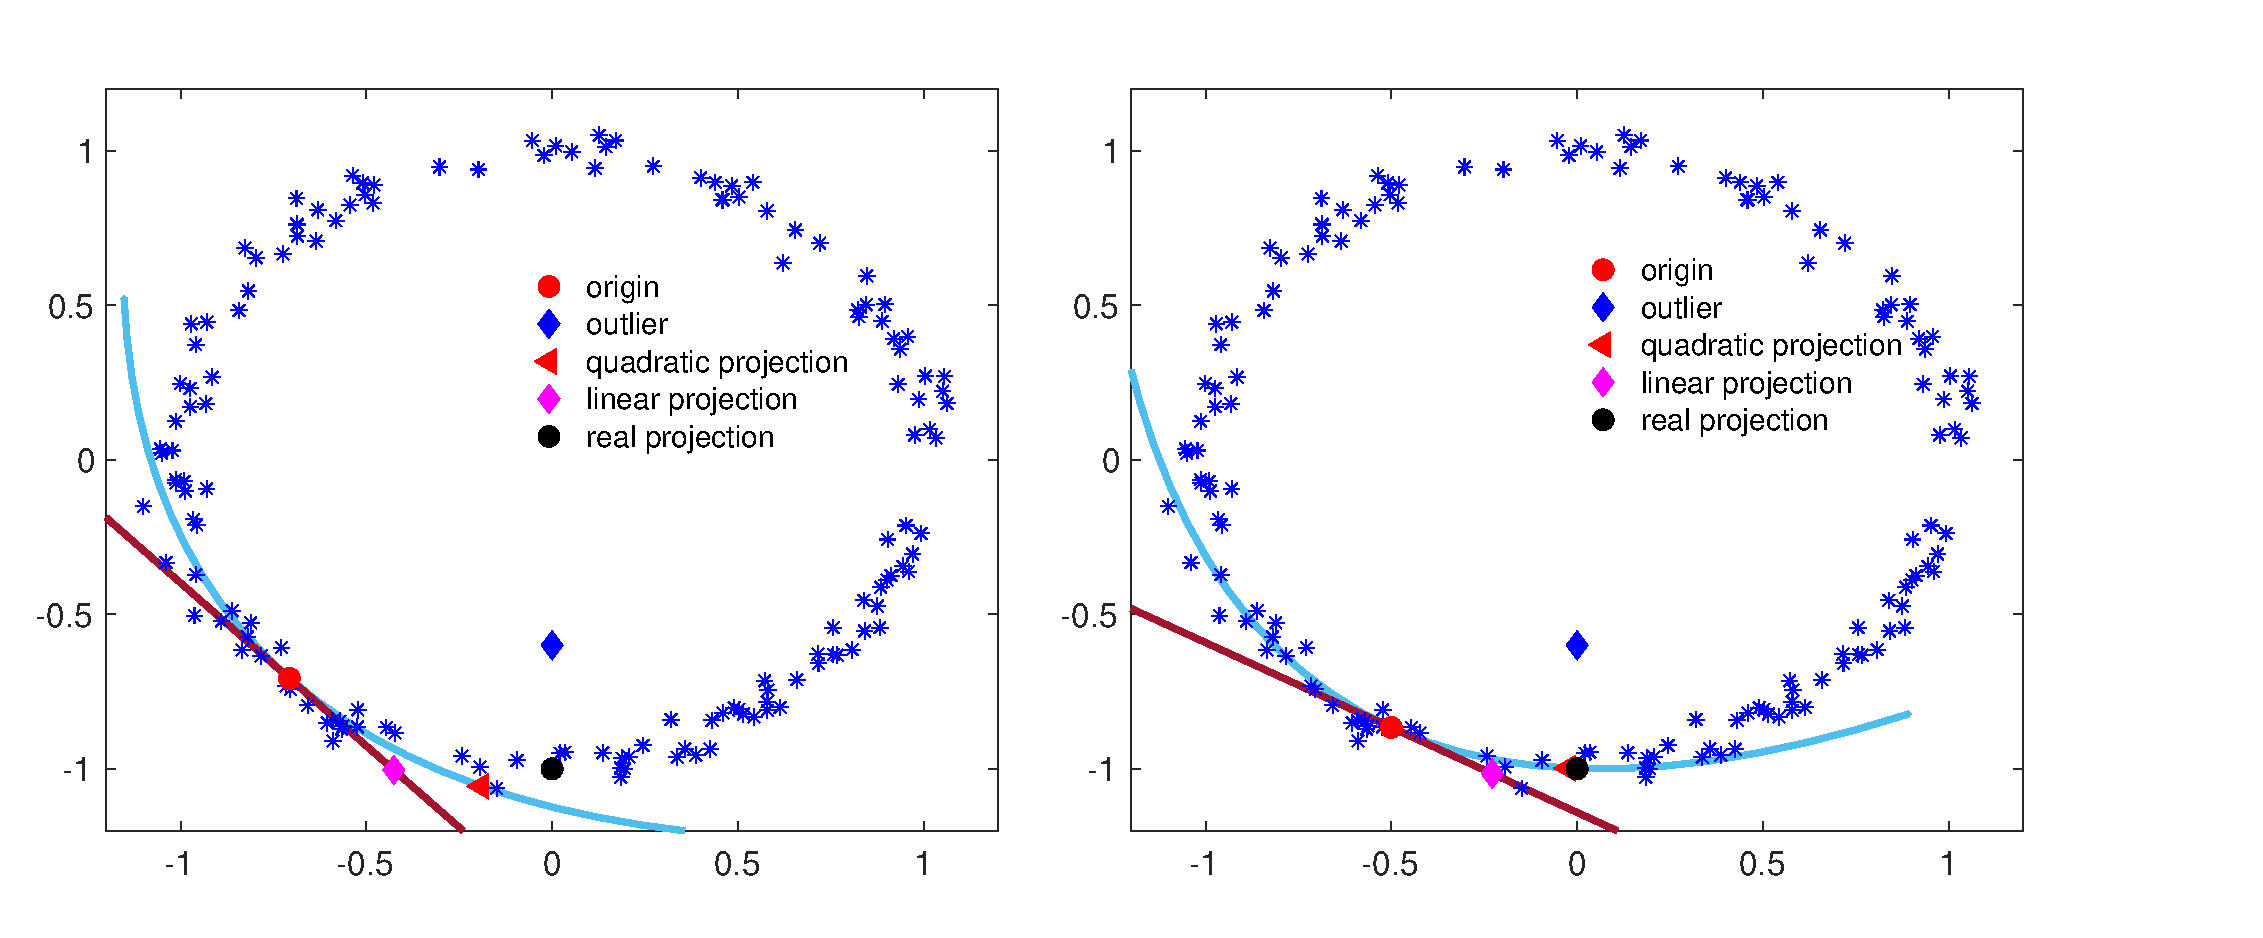
\includegraphics[width=\linewidth]{democ3.eps} 
   \vspace{-0.4cm}
   \caption{The reliance of the origin point in the process of manifold fitting and projection}
   \label{Comparison}
\end{figure}
To demonstrate the difference behaviors corresponding to the linear and quadratic fitting approaches, we give a toy fitting case in Figure \ref{Comparison} with different origins. The origin $x_0$ (the red dot) in the left figure is farther away from the true projection (the black dot) than that in the right figure.  This example shows the effect of the different fitting errors, which is $O(\|\tau\|_2^2)$ and $O(\|\tau\|_2^3)$ corresponding to the linear and quadratic forms, respectively. From this case, we know that the linear approach relies on a good origin heavily than the quadratic form because the approximation by linear case yields a lower-order error comparing with the quadratic case.
 

In this paper, we transfer our manifold fitting problem into finding an approximation version of $\phi_{x_0}(\tau)$ through a deep analysis on the characteristic of it. We also show the dominant term for Taylor expansion of $\phi_{x_0}(\tau)$ can be written as a quadratic form of a tensor acting on $\tau$, i.e, $\nabla\nabla \phi_{x_0}(\tau)|_{\tau=0}(\tau,\tau)$, where $\nabla\nabla\phi_{x_0}(\tau)|_{\tau=0}$ is a third-order tensor with shape of $d\times d\times (D-d)$.  

In addition, we show that, by adopting the dominant term in the Taylor expansion of $\phi_{x_0}(\tau)$,  the nonlinear function $\phi_{x_0}(\tau)$ can be locally simplified as a quadratic form of ${\cal A}(\tau,\tau)$, where $\cal A$ is the empirical estimation of $\nabla\nabla \phi_{x_0}(\tau)|_{\tau=0}$. The unknown parameters $\cal A$ can be obtained via solving a linear least square problem. After obtaining the representation of $x_{\cal A}(\tau)$, we also develop a projection strategy to refine the outlier point $\bar{x}$ by projecting it onto our fitted manifold $\cal M_A$. Furthermore, we show the projection of $\bar{x}$ onto $\cal M_A$ can be achieved by repeatedly solving a series of linear least square problems.
%\section{Related work}
%\subsection{Manifold approximation by Linear Methods}
%Fitting the manifold with linear methods corresponds to setting $\phi_{x_0}(\tau)$ in \eqref{manifold} equals to zero. Then, the problem becomes to find $x_0$ and $U_{x_0}$ such that we can approximate the manifold linear around $x_0$ by a linear parameterization form
%\[
%x(\tau) = x_0 + U_{x_0} \tau
%\]
%Note that, the function $x(\tau)$ is a local approximation of $\cal M$ at $x_0$. The choice of $x_0$ depending on our interest area, such that, if we want to project an outlier $\bar{x}$ onto the manifold, $x_0$ can be selected as the nearest point $x_0$ on $\cal M$, such that 
%\[
%\|x_0-\bar{x}\|_2=\min_{x_0\in \cal M} \|x_0-\bar{x}\|_2
%\]
%
%There are lots of works which approximate the basis $U_{x_0}$ in the tangent space by a linear space approach. 
%One approach is to directly fit the manifold by finding the eigenspace of some matrices, e.g the covariance matrix or Hessian of KDE. Then using the eigenvalue-decomposition to get the eigenspace corresponding to the $d$ largest eigenvalues. The Hessian of the the classical KDE approach shares the same eigenspace of 
%\[
%C(\bar{x}) = \sum_i K_h(\bar{x},x_i) (x_i-\bar{x})(x_i-\bar{x})^T
%\]
%If transformed by the concave increasing function $\log$ with respect to the KDE function, the deterministic term in the Hessian matrix will become 
%\[
%C(\bar{x}) = \sum_i K_h(\bar{x},x_i) (x_i-c(\bar{x}))(x_i-c(\bar{x}))^T
%\]
%where $c(\bar{x})$ is the weighted shift mean vector. In this case, using the basis (consisting of the columns of $U_d$) corresponding to the largest $d$ eigenvalues of the covariance matrix $C(\bar{x})$. 
%
%When we use the locally shift mean to replace the origin $x_0$,  the affine space yields the form as
%\[
%x(\tau) = c(\bar{x}) + U_d\tau,
%\]
%where $\tau$ is the coordinate in the $d$-dimensional space. The projection onto the $x(\tau)$ of $\bar{x}$ is
% \[
%\bar{x}+U_{\perp}U_{\perp}^T(c(\bar{x})-\bar{x}) = c(\bar{x})+ U_dU_d^T(\bar{x} -c(\bar{x}))
%\]
%There are also complex methods such as \cite{fefferman2018fitting,yao2019manifold} by approximating the normal space at $x$ as a weighted combination of the normal space at each neighbor sample $x_i$ as
%\[
%A = \sum_i \alpha_i \Pi_i^{\perp}
%\]
%where $\Pi_i^{\perp}$ is the estimated normal space at the observation $x_i$ and $\alpha_i$ is the weight for $x_i$.
%Then the normal space can be obtained from eigenvalue decomposition of $A$ and picking up the eigenvectors corresponding to the $D-d$ largest eigenvalues.
%%Usually, the normal space (orthogonal complement of the tangent space) is used to act as a constraint, such that, the iteration of the mean-shift algorithm performs within a proper subspace. This subspace constraint tries to keep the component in the normal space and leave out or diminish the component of scale in the tangent space. All the normal space is obtained from the eigenvalue decomposition of a temporary matrix (Hessian or Combination of Normal Space).
%%
%% For the ridges obtained from both SCRE and {log}-SCRE (SCRE transformed with a $\log$ function), we need to compute the second derivative for the function to obtain the Hessian matrix $H(x)$ or the corresponding covariance matrix $J(x)$. Then, the projection can be produced from the eigenvalue decomposition, and we can pick the eigenspace corresponding to the smallest D-d eigenvalues. For SCRE, the covariance matrix is $J(x) = \sum_i w(x_i,x)(x_i-x)(x_i-x)^T$. For {log}-SCRE, the covariance matrix is $J(x) = \sum_i w(x_i,x)(x_i-c(x))(x_i-c(x))^T$, where $c(x)$ is the one-step shift mean of $x$.
%%
%% In our {\it l}-SCRE approach, we build the semidefinite local covariance matrix as $C_{r}(x)=\sum_{i\in {\cal I}_r} w_{h,r}(x_i, x)(x_i-c_r(x))(x_i-c_r(x))^T$. The {\it l}-SCRE has two main advantages. First, the covariance matrix $C_{r}(x)$ in the local area of $B_{{x}}(r)$ is more similar to a low-rank matrix than one in a global area. As a result, we can easily recover the low-dimensional space to approximate $B_{{x}}(r)\cap \mathcal M$. Second, because we restrict our consideration to a small domain, the smooth parameter $h$ can be chosen more easily than before.
%%
%%Instead of computing the Hessian, the manifold-fitting strategy \cite{fefferman2018fitting}  approximates the normal space at ${x}$ with a weighted combination of projection matrix $\Pi_i^{\perp}$ as $A = \sum_i \alpha_i \Pi_i^{\perp}$ of the normal projection $\Pi_i^{\perp}$ at each point $x_i$ in the neighborhood. Then, the D-d principal components from the eigenvalue decomposition of $A$ is regarded as the projection onto the normal space at ${x}$. The benefit of this approach is that the projection $\Pi_i^{\perp}$ at each point $x_i$ is a constant matrix that does not depend on the location of ${x}$. However, because it is required to approximate a large number of tangent spaces, this approach needs  a considerably large amount of computation resources.
%\subsection{Manifold approximation by Nonlinear Least-square Approach}
%Using the moving least-square (MMLS) projection approach to approximate the manifold is proposed by \cite{sober2019manifold}. In their work, they choose to approximate the manifold with two steps. 
%\begin{itemize}
%\item[1.] Given the outlier $x$, find the local coordinates by solving a minimization problem
%\[
%(\hat{q}(x),\hat{\cal H}(x))= \arg\min_{x-q\perp {\cal H}}  
% \sum_{i=1}^n d^2 (x_i, {\cal H}) \theta(\|x_i-q\|),
%\]
%where $\cal H$ is the $d$-dimensional affine subspace and $q$ is the origin. The squared distance from $x_i$ to $\cal H$ is $d^2 (x_i, {\cal H}) = \|V^T_{\cal H}(x_i -q)\|_2^2$.
%The parameter $\hat{q}$ and $\hat{H}$ is achieved by a repeated minimizing procedure. 
%
%\item[2.]  Using the local coordinate $\tau_i = V^T_{\cal H}(x_i-q)$, fit the polynomial by minimizing
%\[
%\hat{g} = \min_{p\in \Pi_m^d} \sum_{i=1}^n \|p(\tau_i)-f_i\|_2^2 \theta(\|x_i-q\|),
%\]
%where $\Pi_m^d$ is the polynomial function class up to order $m$ defined in the $d$-dimensional space. Then, the projection is defined as: $P_m(r) = \hat{g}(0)$. 
%\end{itemize}
%\subsection{Difference}
%Our approach differ with the former approaches in three respects. 
%\begin{itemize}
%\item[1.] We do not require the origin satisfy $r-q\perp H$ in our approach by simplifying the first step. 
%%by give a initial $q$ as the origin of our fitting. 
%Since our method is not sensitive to the initial point $q$, by using the initial guess of $q$, $H$ can be obtained by PCA very easily.
%\item[2.] We restrict the form of our polynomial which will result in a with very concise form and save lots of extra parameters. The manifold fitting by a second-order paraboloid function has a more concrete form by defining a tensor which has the clear meaning by representing the curvature of our manifold. The tensor can be obtained by solve a linear least square problem in each of the normal dimensions.
%\item[3.] The projection of outlier $r$ onto the fitted manifold $\cal M_A$ is not restraint to be the origin point of ${\cal M_A}$. It can be any points $\cal M_A$ as long as the minimum criteria is achieved.
%\end{itemize}
The strengths of our method can be summarized as:
%\begin{itemize}

1. By fitting a function with the quadratic form, the curvature of the manifold is considered in our algorithm. Because of the existing of the curvature, the fitted manifold ${\cal M}_{\cal A}$ can approximate the true manifold in a relatively larger scope.

2. Our algorithm does not rely on the accuracy of the estimated origin point too much, which means a relatively rough estimation of the origin is accessible in our algorithm. Instead of the origin, we just need to get a point (nearby $x$) which is also supposed to be next to the true $\cal M$.

3. The solution of our algorithm has a clear geometric interpretation via the optimized $\hat{\tau}$.  When we got the local coordinate $\hat{\tau}$, we can think of our projected point $x(\hat{\tau})$ ( the projection onto ${\cal M}_{\cal A}$) as a modification of the origin $x_0$, through,
\[
x(\tau) = U_\perp {\cal A}(\tau,\tau) + U\tau + x_0. 
\]
where $U\tau$ is the modification of $x_0$ in the tangent space and ${\cal A}(\tau,\tau)$ is the modification of $x_0$ in the normal space.
%\end{itemize}
%\section{Preliminary: Tensor Operation} 
%In this section, we give some preliminary knowledge with tensor operation and tensor differentiation. Using tensor notations  will bring in lots of convenience in our notations and discussion.
%\subsection{Multiplication}
%For a three-order tensor $\cal A$ with the shape of $d\times d\times (D-d)$, 
%%As the matrix can be seen as a tensor of order 2. 
%we can also think of $\cal A$ as an operator acting on the $d$ or $(D-d)$ dimensional vector space, besides regarding $\cal A$ as a particular array of numbers.
%For a vector $\tau \in {\mathbb R}^d$, the tensor $\cal A$ acting on $\tau$ will result in a matrix denoted as ${\cal A}(\tau)$ of shape $d\times (D-d)$, of which the $j,k$-th element is
%\[
%\{{\cal A}(\tau)\}_{jk} = \sum_i \tau_i {\cal A}_{i,j,k},
%\]
%which is a weighted combination of the slices in the first dimension of the tensor $\cal A$.
%Similarly, for two vectors $\tau,\eta\in {\mathbb R}^d$, the tensor $\cal A$ acting on $\tau,\eta$ will result in a vector denoted as ${\cal A}(\tau,\eta)\in {\mathbb R}^{D-d}$, whose $k$-th element is
%\[
%\{{\cal A}(\tau,\eta)\}_{k} = \sum_{i,j} \tau_i \eta_j {\cal A}_{i,j,k} .
%\]
%Clearly, we have the vector ${\cal A}(\tau,\eta)$ can be written as a matrix-vector product by: $ {\cal A}(\tau,\eta) = {\cal A}(\tau)^T \eta$ and the summation with index $i,j$ can also be regarded as an inner product of matrix, i.e, $\{{\cal A}(\tau,\eta)\}_{k}=\langle\tau\eta^T ,{\cal A}_{\cdot\cdot k}  \rangle $ .%, where ${\cal A}(\tau)^T \eta$ is the ordinary matrix-vector multiplication.
%\subsection{Differentiation}
%For the $(D-d)$ dimensional vector ${\cal A}(\tau,\tau)$, we can take the differential operation with respect to $\tau$. The first derivative of ${\cal A}(\tau,\tau)$ with respect to $\tau$ will result in a matrix of size $d\times (D-d)$ and the second derivative of ${\cal A}(\tau,\eta)$ with respect to $\tau$ and $\eta$ will get the tensor $\cal A$,
%\begin{gather*}
%\nabla_\tau {\cal A}(\tau,\tau) =  2{\cal A}(\tau) \in \mathbb{R}^{d\times (D-d)},\\
%\nabla_\eta \nabla_\tau {\cal A}(\tau,\eta) =  {\cal A}\in  \mathbb{R}^{d\times d\times (D-d)},\\
%\nabla_\tau \nabla_\tau {\cal A}(\tau,\tau) =  2{\cal A}\in  \mathbb{R}^{d\times d\times (D-d)}.
%\end{gather*}
%Noticing that ${\cal A}(\tau,\tau,\iota)$ is a scalar, taking the derivative for $\tau$ twice will result in a symmetric matrix (similar with Hessian)
%\begin{gather*}
%\nabla_\eta \nabla_\tau {\cal A}(\eta,\tau,\iota) =  {\cal A(\iota)} = \sum_k \iota_k {\cal A}_{\cdot\cdot k}\in \mathbb{R}^{d\times d},\\
%\nabla_\tau \nabla_\tau {\cal A}(\tau,\tau,\iota) =  2{\cal A(\iota)} = 2\sum_k \iota_k {\cal A}_{\cdot\cdot k}\in \mathbb{R}^{d\times d},
%\end{gather*}
%where ${\cal A(\iota)}$ is a matrix obtained via folding the tensor in the third dimension with the weight $\iota$, i.e, the $i,j$-th element is:
%\[
%{\cal A(\iota)}_{i,j} = \sum_k \iota_k  {\cal A}_{i,j,k}.
%\] 
%
%The tensor multiplication operations and differentiations will be used frequently in our manifold projection section of this manuscript. Working with the tensor can make our writing more concise.
\section{Fitting Model}
There are two meanings of the fitting model. The first refers to locally fitting a complicated function by a simple form such as Taylor expansion. The second indicates we use a generalized representation such that the measurement with respect to the observations and the representation is optimal under some criteria.  

For a complicate nonlinear function $\phi(\tau)$, we can fit locally via the lower order Taylor expansion such as
\begin{equation}\label{quadratic_f}
\begin{aligned}
\phi_q(\tau) = &\phi(\tau_0) + \langle \nabla_\tau \phi(\tau)|_{\tau=\tau_0}, \tau-\tau_0 \rangle +...\\
&+ \frac{1}{2} \nabla_\tau \nabla_\tau \phi(\tau)|_{\tau=\tau_0} (\tau-\tau_0,\tau-\tau_0).
\end{aligned}
\end{equation}
%\begin{itemize}

1. The linear function
$
\phi(\tau_0) + \langle \nabla_\tau \phi(\tau)|_{\tau=\tau_0}, \tau-\tau_0 \rangle
$ 
can be thought as a locally fitting model of $\phi(\tau)$ at $\tau=\tau_0$ with the error of order $O(\|\tau-\tau_0 \|_2^2)$.

2. The quadratic function \eqref{quadratic_f} can be thought as a locally fitting model of $\phi(\tau)$ at $\tau=\tau_0$ with the error of order $O(\|\tau-\tau_0 \|_2^3)$.
%\begin{equation}\label{quadratic_f}
%\phi(\tau_0) + \langle \nabla_\tau \phi(\tau)|_{\tau=\tau_0}, \tau-\tau_0 \rangle+\frac{1}{2} \nabla_\tau \nabla_\tau \phi(\tau)|_{\tau=\tau_0} (\tau-\tau_0,\tau-\tau_0)
%\end{equation}
%\end{itemize}
In this paper, we solve the manifold fitting problem via the local quadratic approximation under the noisy observations. To simplify the problem, we first assume:
%\begin{assumption}
%Assume the observations $\{x_i, i=1,...n\}$ and the origin $x_0$ are drawn exactly from some unknown $d$-dimensional manifold $\cal M$ which is embedded in the $D$-dimensional ambient space.
% %Assume to fit a $d$-dimensional manifold $\cal M$ embedding in the ambient space ${\mathbb R}^D$. No noise considered. i.e, the data are drawn from the manifold and the fitting point $x_0$ also on the manifold.
%%\end{itemize}
%\end{assumption}

\subsection{Quadratic surface in 3-D space}
A manifold is a topological space that locally resembles Euclidean space. Except for a few special cases, we cannot have global representation to parameterize the manifold. As a result, we try to approximate the manifold locally within an interested area. First, we provide a simple demo as an illustration.
\begin{example}
\begin{figure}[H] %  figure placement: here, top, bottom, or page
   \centering
   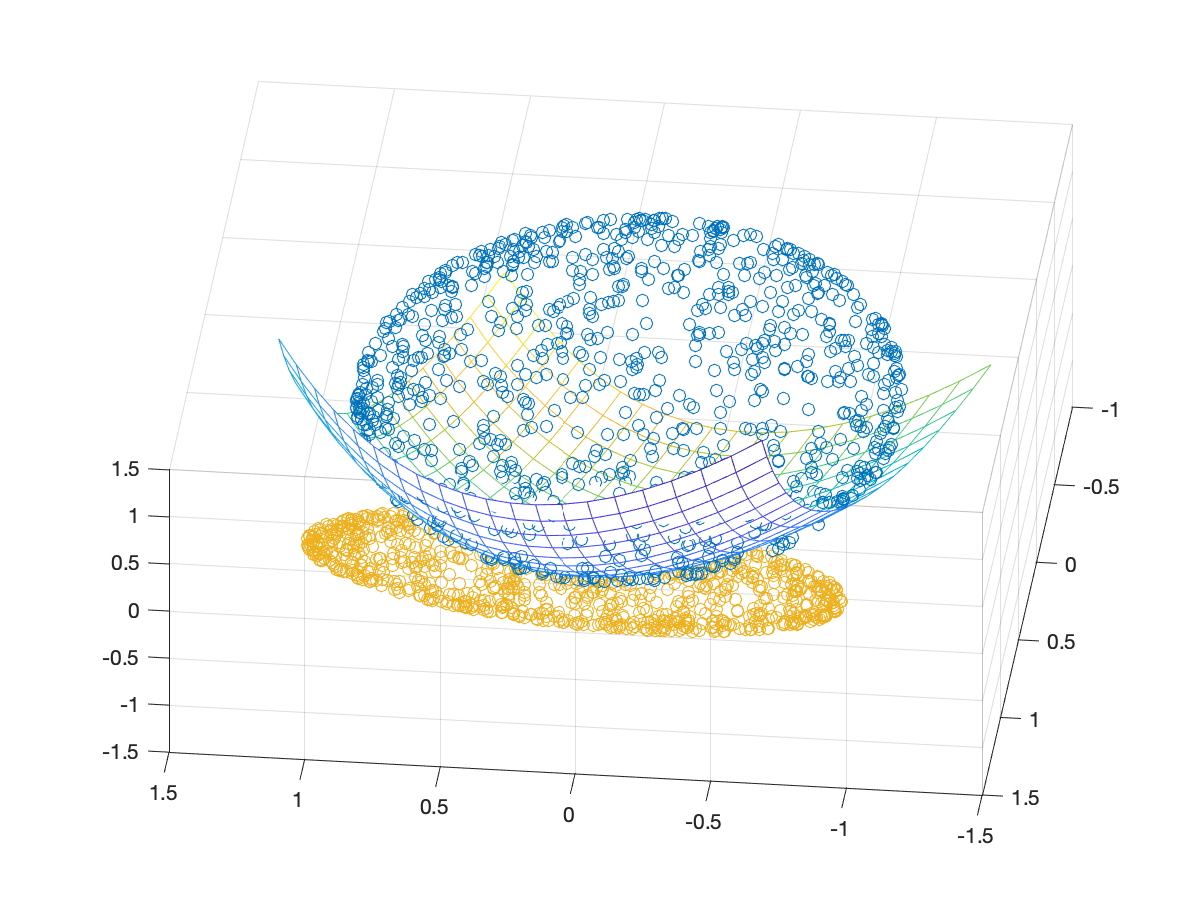
\includegraphics[width=0.7\linewidth]{demo.eps} 
   \vspace{-0.4cm}
   \caption{Fitting a manifold with the elliptical paraboloid surface}
   \label{3-D paraboloid}
\end{figure}
%We give an example by constructing a fitted paraboloid surface in 3-dimensional Space.
The data, consisting of blue circles evenly distributed on a 2-D sphere as shown in \eqref{3-D paraboloid}, is a toy example of a manifold. Fixing a point $x_0\in {\mathbb S}^2$, we can have a tangent plane. The yellow circles are the projection of the data onto the tangent plane. The continuous elliptical paraboloid surface is the structure we want.
%As shown in the Figure \eqref{3-D paraboloid}, the yellow circle $\circ$ is the projection of the points from the 3-dimensional ball onto the tangent space. The mesh surface is the fitted structure to locally approximate the manifold (3-dimensional ball). 
Figure \ref{3-D paraboloid} clearly shows that the mesh surface is a better structure to approximate $\mathbb{S}^2$, compared with the tangent plane. Here, the parameterized function of the quadratic form  $x_A(\tau): {\mathbbm R}^2\rightarrow {\mathbbm R}^3$ yields:
$
x_A(\tau) = x_0 + U_{x_0} \tau + {U_{x_0}^\perp} \tau^T A \tau,
$
where $A$ is a matrix of size $2\times 2$ that is used to control the shape and direction of the paraboloid surface. The eigenvalues of $A$ represent the curvature or flatness in the corresponding eigenvector direction.
\end{example}
%\remark{In 3-D space, obviously, 
%when the paraboloid surface is at one side of the tangent plane, the matrix $A$ is positive definite or negative definite.
%}
\subsection{Quadratic surface in high-dimensional space }

 Instead of fitting the manifold via the tangent plane, we bring a unknown function $\phi_{x_0}(\tau)$ from the tangent space to the normal space
 \[
 \phi_{x_0}(\tau): {\mathbbm R}^d \rightarrow {\mathbbm R}^{D-d}.
 \] 
 Using  $\phi_{x_0}(\tau)$, we know any manifold $\cal M$ that is local at $x_0$ can be written as the range of  function  $x(\tau)$:
  \begin{equation}\label{model}
  x (\tau)=  x_0 + U_{x_0} \tau+ U_{x_0}^{\perp} \phi_{x_0} (\tau),
  \end{equation}
where $\phi_{x_0}(\tau)=[\phi_{x_0}^{d+1}(\tau),...,\phi_{x_0}^{D}(\tau)]^T$  is the function from tangent space to the normal space. $\tau$ is the local coordinate in the tangent space.
From \eqref{model}, we know that there is a one-to-one correspondence between $\phi_{x_0} (\tau)$ and $x(\tau)$: %(equivalent to)
\begin{equation}\label{phi}
\phi_{x_0}(\tau) = {U_{x_0}^{\perp}}^{T}(x(\tau)-x_0)
\end{equation}
From \eqref{phi}, we know that, if we are given the structure of $\phi_{x_0}(\tau)$ with some parameters, we can have the representation of $\phi_{x_0}(\tau)$, for the following reasons:
%\begin{itemize}

1. $x_0$ is any point on the manifold we are interested in.

2.  $U_{x_0}$ is the basis of principal space at $x_0$, which can be obtained from the local PCA. $U_{x_0}^{\perp}$ is the orthogonal direction at $x_0$, which can also be obtained from the local PCA.

3. The only remaining part is  $\phi_{x_0} (\tau)$.

%\end{itemize}
Note that, to implement the local PCA, the local covariance matrix at $x_0$ is defined as $C(x_0) = \sum_i K_h(x_0,x_i) (x_i-x_0)(x_i-x_0)^T$. The basis of the estimated tangent space can be obtained from the eigenvalue decomposition:
\begin{equation}\label{eign-decom}
C(x_0) = [U_d , U_{D-d}] 
\left[
\begin{array}{cc}
\Lambda_1& 0\\
0 & \Lambda_2
\end{array}\right]
 [U_d , U_{D-d}]^T.
\end{equation}
From the decomposition in \eqref{eign-decom}, we can set the basis on the tangent plane as $U_{x_0} = U_d$, and the basis on the normal space as $U_{x_0}^\perp = U_{D-d}$. In the local domain ${\mathbb R}_{x_0}^D (r)\cap \cal M$,  $\phi_x(\tau)$ can be approximated by the polynomial of order two. Thus, we will get
\begin{equation}\label{app_phi}
\begin{aligned}
\phi_{x_0}(\tau) =& \phi_{x_0}(0)+ \nabla {\phi_{x_0}}(\tau)|_{\tau=0}(\tau)+ \\
&+\frac{1}{2}{\nabla\nabla\phi_{x_0}(\tau)|_{\tau=0}}(\tau, \tau)+O(\|\tau\|_2^3),
\end{aligned}
\end{equation}
where ${\nabla\nabla\phi_{x_0}(\tau)|_{\tau=0}}$ stands for the second fundamental form, which is a three-order tensor of size $ d\times d\times (D-d)$. Acting on $\tau$ twice will result in a vector of size $D-d$.  The linear gradient operator  $\nabla {\phi_{x_0}}(\tau)|_{\tau=0}\in \mathbb{R}^{{(D-d)}\times d}$ acting on $\tau$ will result in a vector in the normal space of size $D-d$.

%\begin{theorem}\label{tangent property}
%If the columns of $U_{x_0}$ consist of  the basis of tangent space of $\cal M$ at $x_0$, then, the nonlinear function $\phi_{x_0}(x)$ satisfies:
%\[
%\phi_{x_0}(0) = 0,\quad \nabla {\phi_{x_0}}(0) = 0.
%\]
%\end{theorem}
%\begin{proof}
%Recall that: $x (\tau)=  x_0 + U_{x_0} \tau+ U_{x_0}^{\perp} \phi_{x_0} (\tau)$. Let $\tau = 0$, then, we have
%\[
%U_{x_0}^{\perp} \phi_{x_0} (0) = 0
%\]
%Because of $U_{x_0}^{\perp}$ is a orthonormal matrix, $U_{x_0}^{\perp} \phi_{x_0} (0) = 0$ implies $\phi_{x_0} (0)=0$.
%
%For any curve $\gamma(t)\in {\mathbbm R}^d, \gamma(0) = 0, \gamma'(0)=v$.
%If we take the direction derivative for $x(\tau)$:
%\[
%\begin{aligned}
%&\partial_v x(\tau)   = \frac{d x(\gamma(t))}{dt}|_{t=0} = \lim_{t\rightarrow 0} \frac{x(\tau+vt)-x(\tau)}{t}\\
%=& \lim_{t\rightarrow 0} \frac{U_{x_0}(\tau+tv) -U_{x_0}(\tau)+U_{x_0}^{\perp} \phi_x(\tau+tv)-U_{x_0}^{\perp} \phi_x(\tau)}{t}\\
%=&U_{x_0} v + U_{x_0}^{\perp} \nabla{\phi_x}(\tau) v
%\end{aligned}
%\]
%Because  $\partial_v x(\tau)\in {\cal T}_{\cal M}({x_0})$, we have $U_{x_0}^{\perp} \nabla{\phi} (\tau)\in {\cal T}_{\cal M}({x_0})$. Thus, we have
%\[
%U_{x_0}^{\perp} \nabla {\phi} (\tau)= 0,
%\]
%which implies $ \nabla {\phi} (\tau)=0$ because the columns of the orthonormal matrix $U_{x_0}^{\perp}$ are linear independent .
%\end{proof}
Recalling that \eqref{app_phi}, we know $\cal M$ can be parameterized with the remainder term:
\[
 x(\tau)= x_0+ U_{x_0} \tau + \frac{1}{2} U_{x_0}^{\perp}{\nabla\nabla\phi_{x_0}(\tau)|_{\tau=0}}(\tau, \tau)+O(\|\tau\|_2^3)
\]
For notational convenience, we denote the tensor as ${\cal A}=\frac{1}{2} {\nabla\nabla\phi_{x_0}(\tau)|_{\tau=0}}$ and define a function $x_{\cal A}(\tau)$ related with $\cal A$ as
\begin{equation}\label{fun_range}
x_{\cal A}(\tau) = x_0+ U_{x_0} \tau + U_{x_0}^{\perp} {\cal A}_{\phi_{x_0}}(\tau, \tau).
\end{equation}
From the range $x_{\cal A}(\tau)$ of \eqref{fun_range}, we have a new manifold ${\cal M_A}$ derived from $x_{\cal A}(\tau)$ as
\begin{equation}\label{M_a}
{\cal M_A} = \{ z| z =  x_0+ U_{x_0} \tau + U_{x_0}^{\perp} {\cal A}_{\phi_{x_0}}(\tau, \tau), \tau \in {\mathbb R}^d\}
\end{equation}
%From \eqref{M_a}, we know ${\cal M_A}$ is derived from 
%\[
%x_{\cal A}(\tau) = x_0+ U_{x_0} \tau + U_{x_0}^{\perp} {\cal A}_{\phi_{x_0}}(\tau, \tau).
%\]
Because of $x_{\cal A}(\tau)-x(\tau) = O(\|\tau\|_2^3)$, we know ${\cal M_A}$ approximates $\cal M$ well when the scale of  $\tau_i$ is relatively small.
%\subsection{Paraboloid Surface}
%Define the paraboloid surface function at $x_0$ to be
%\begin{equation}\label{Paraboloid}
%\psi(\tau, {\cal A}_{\phi_{x_0}}) = x_0+ U_{x_0} \tau + U_{x_0}^{\perp} {\cal A}_{\phi_{x_0}}(\tau, \tau).
%\end{equation}
%We use it to fit manifold at a local domain of $R_{x_0}^D \cap \cal M$. From now on, if we don't need to emphasize the function $\phi_{x_0}$, we abbreviate ${\cal A}_{\phi_{x_0}}$ as $\cal A$ to represent the three order tensor.

%Note, that the range of $\psi(\tau)$ is a quadric approximation of manifold $\cal M$. 
In most of the manifold fitting cases, both of the true manifold $\cal M$ and the function $\phi_{x_0}(\tau)$ are unknown, as a result, it is impossible for us to get the second order parameter ${\cal A}_{x_0}$ through differentiating the multivariable function $\phi_{x_0}(\tau)$.
Instead of getting the accurate $\phi_{x_0}(\tau)$, we can estimated it by using the data (observations) which is supposed to be drawn from some low-dimensional manifold. In this case, we need to estimate the ${\cal A}_{\phi_{x_0}}$ from the observations to obtain $\hat{\cal A}$, as a result, the range $\cal M_{\hat{\cal A}}$ of $x_{\hat{\cal A}}(\tau)$ can be assumed a local smoothed approximation of $\cal M$ around $x_0$ to some degree.
From now on, we will abbreviate $\hat{\cal A}$ as ${\cal A}$, to stand for the estimated second order parameter.
\subsection{Fitting Model}
In real case, when we have samples from the manifold, we need to determine  $U_{x_0}, {\cal A}_{\phi_{x_0}}(0)$ by knowing $x_0, \{x_i\}$.
Using local principal analysis, we know for each observation $x_i$, there is a local coordinate $\tau_i = \tau(x_i,x_0, U_{x_0})$ in the tangent space. When we use $x_0$ as the origin of the coordinate. By projecting onto the tangent space, we have the local coordinate has the closed-form solution as
\begin{equation}\label{tangent_coor}
\tau_i = U_{x_0}^T (x_i -x_0).
\end{equation}
When having $\{\tau_i, U_{x_0}, x_0\}$, we can determine the tensor $\cal A$ by a least square problem. The global coordinate $x_i$ has a second order approximation as
\begin{equation}\label{x_tau}
 x_i  -  (x_0+ U_{x_0} \tau_i + U_{x_0}^{\perp} {\cal A}(\tau_i,\tau_i)) = o(\|\tau_i\|_2^2).
\end{equation}
%where we can split the tensor acting on $\tau_i$ as
%\[
%{\cal A}_{\phi_{x_0}}(0)(\tau_i,\tau_i) = [\tau_i^T S^{d+1}\tau_i, ...,\tau_i^T S^{D}\tau_i]^T.
%\]
We should find a tensor $\cal A$ such that the remainder is a higher-order item.
%\begin{equation}\label{optimA}
% \|x_i  -  (x_0+ U_{x_0} \tau_i + U_{x_0}^{\perp} {\cal A}(\tau_i,\tau_i)) \|_2^2
%\end{equation}
Substitute \eqref{tangent_coor} into \eqref{x_tau}, we have
\[
\begin{aligned}
 &x_i  -  (x_0+ U_{x_0} \tau_i + U_{x_0}^{\perp} {\cal A}(\tau_i,\tau_i))\\
 =&U_{x_0}^\perp( {U_{x_0}^\perp}^T (x_i -x_0) -{\cal A}(\tau_i,\tau_i) )= o(\|\tau_i\|_2^2),
 \end{aligned}
\]
which is equivalent to 
\begin{equation}\label{normal_appro}
 {U_{x_0}^\perp}^T (x_i -x_0) -{\cal A}(\tau_i,\tau_i) = o(\|\tau_i\|_2^2).
\end{equation}
%For \eqref{phi}, we can get the best estimated value of ${\cal A}_{\phi_{x_0}}(0)(\tau_i,\tau_i) $ as
%\begin{equation}\label{all-dimension}
%{U_{x_0}^\perp}^T (x_i -x_0)  = \hat{\cal A}_{\phi_{x_0}}(0)(\tau_i,\tau_i)  + o(\|\tau_i\|_2^2)
%\end{equation}
Noticing that \eqref{normal_appro} is a vector form, split \eqref{normal_appro} into each dimension, e.g, for the $k$-th dimension in the normal space, we have
\begin{equation}\label{normal_approx}
\begin{aligned}
 {(u^k_{x_0})}^T (x_i -x_0) 
=&{\cal A}_{\cdot\cdot k}(\tau_i,\tau_i) +  o(\|\tau_i\|_2^2)\\
=&\tau_i^T S^{k}\tau_i + o(\|\tau_i\|_2^2).
\end{aligned}
\end{equation}
In \eqref{normal_approx}, because of the symmetric position of $\tau_i$, we know that the best fitted $S^k$ is symmetric, i.e, each slice of ${\cal A}_{\cdot\cdot k}$ is a symmetric matrix. Therefore, the unknown parameters in $S^k$ yields a total number of ${d(d+1)}/{2}$. 

%In \eqref{normal_approx}, the only unknown is $\cal A$, finding the best approximation of $\cal A$ in the $\|\cdot\|_2^2$ criteria is a linear regression or least square problem. To use the linear algebra tools, we should vectorize each slice of $\cal A$.

In the following section, we will show how to vectorize each slice of $\cal A$ and  how to make the vectorized result into the matrix form. Also, we show the quadratic form equals to the inner product of two vectors as
\[
\tau_i^T S^{k}\tau_i  = 2{\rm vech}(\tau_i\tau_i^T,1)^T {\rm vech}(S^k,1/2).
\]

\subsection{Closed-form of $S^k$ by Vectorization}
%In this section, we vectorize the matrix, such that we could obtain $S^k$ by using a least square problem with samples $\{x_i\}$.
For any symmetric matrix $A$, we know $A_{ij} = A_{ji}$. Therefore, we can only need ${d(d+1)}/{2}$ elements with the corresponding order to restore it. As a result, we can only vectorize the upper-triangle elements in the matrix $A$ as a vector 
\[
{\rm vech}(A,t)_{\frac{(2d-i)(i-1)}{2}+j-i+1} = \left\{
\begin{array}{cc}
A_{ij},    &\quad j>i\\
tA_{ij},   &\quad j=i,
\end{array}
\right.
\]
where the diagonal elements multiplied by a scalar $t$, which will bring us convenience for our following notations. When $t=1$, the vector is constructed by picking the upper-triangle elements of $A$ including the diagonal ones, i.e., 
\[
{\rm vech}(A,1) = [A_{11},A_{12},...A_{1d},...A_{dd}]^T.
\]
When $t=1/2$, the vector is constructed by picking the upper-triangle elements of $A$, and half of the diagonal elements, i.e.,
\[
{\rm vech}(A,{1}/{2}) = [A_{11}/2,A_{12},...A_{1d},...A_{dd}/2]^T.
\]
%Here, the vectorization operates with the elements in ${\rm vech}(A,1)$ and $A$ yield a relation as:
%\begin{gather*}
%{\rm vech}(A,1)_{\frac{(2n-i)(i-1)}{2}+j-i+1} = \left\{
%\begin{array}{cc}
%A_{ij},    &\quad j>i\\
% A_{ij},&\quad j=i
%\end{array}
%\right.\\
%{\rm vech}(A,1/2)_{\frac{(2n-i)(i-1)}{2}+j-i+1} = \left\{
%\begin{array}{cc}
%A_{ij},    &\quad j>i\\
% A_{ij}/2,&\quad j=i
%\end{array}
%\right.
%\end{gather*}
%Notice that $\theta_k$ is obtained by selecting the upper-triangle elements of $S^k$. 
Note that, we can easily recover the matrix $A$ from the vector ${\rm vech}(A,1/2)$ by
%Conversely, we can also recover $S^k$ from $\theta_k$, by
\[
A = {\rm Mat} ({\rm vech}(A,1/2)) + {\rm Mat}^T ({\rm vech}(A,1/2)) 
\]
where ${\rm Mat}(y)$ is an operator constructed by realigning the elements in $y$ into an upper-triangle matrix ${\rm Mat} (y)$ such that the $i,j$-th elements equals to
\[
{\rm Mat} (y) _{i,j} =\left\{
\begin{array}{cc}
 y_{{(2d-i)(i-1)}/{2}+j-i+1},& j\geq i\\
 0,& j<i
\end{array}
 \right.
\]
With the above notations, the quadratic form $x^T A x$ can be written in the vectorized version as
\[
x^T A x = 2{\rm vech}(xx^T,1)^T {\rm vech}(A,1/2),
\]
where ${\rm vech}(xx^T,1)$ is a vectorization of the symmetric matrix $xx^T$ including the diagonal ones.
%\remark{The vectorization process for a symmetric matrix is invertible, i.e, if we vectorize a symmetric matrix into a vector, we can also turn the vector into a matrix which is identical with the former one.}



%We can vectorize the matrix $\tau_i \tau_i^T$ by placing the upper-triangle of elements in $\tau_i \tau_i^T$ into a vector $g_i$ by
%\[
%g_i  =  [{\tau_i}_{1}^2, {\tau_i}_{1}{\tau_i}_{2},...,{\tau_i}_d^2]^T, 
%\]

%For notational convenience, we denote $\theta_k = {\rm vech}(S^k)$. 
Because of the symmetric of the matrix $\tau_i\tau_i^T$ and $S^k$, using the above notations, it can be easily verified that
\[
\tau_i^TS^k\tau_i = \langle \tau_i\tau_i^T, S^k\rangle =2{\rm vech}(\tau_i\tau_i^T,1)^T {\rm vech}(S^k,1/2).%= 2 \theta_k^T g_i.
\]
For notational convenience, we denote $\theta_k = {\rm vech}(S^k,1/2)$ and $g_i = {\rm vech}(\tau_i\tau_i^T,1)$.
Using the vector notations, the equation in \eqref{normal_approx} can be converted as:
\begin{equation}\label{g_i}
g_i^T \theta_k  - \frac{1}{2}{(u^k_{x_0})}^T (x_i -x_0) = o(\|\tau_i\|_2^2).
\end{equation}
For notational convenience, we use $z_i^k$ to stand for the local coordinate in the $k$-th normal dimension corresponding to $x_i$, i.e.,
\[
z_i^k =  \frac{1}{2}{(u^k_{x_0})}^T (x_i -x_0). %+ o(\|\tau_i\|_2^2).
\] 
From \eqref{g_i}, we know that
$
g_i^T \theta_k  - z_i^k= o(\|\tau_i\|_2^2).
$
To determine the ${d(d+1)}/{2}$ parameters in $\theta_k$, we need ${d(d+1)}/{2}$ linear independent equations. In other words, we need at least ${d(d+1)}/{2}$ samples to construct ${d(d+1)}/{2}$ linear independent $\{g_i, i = 1,...,{d(d+1)}/{2}\}$. 

Suppose, we have $m$ samples on the manifold. Denote the matrix $G$ and the vector $\ell_k$ as
\[
G = [g_1,...,g_m]^T, \quad \ell_k = [z_1^k,..., z^k_m ]^T.
\]
%\remark{ Idealy, we only need ${d(d+1)}/{2}$ samples to fix $\{S^k,k=d+1,D\}$ if and only if the rows of $G$ can span the whole space of the ${{d(d+1)}/{2}}$-dimensional space, i.e. ${\rm rank}(G)={d(d+1)}/{2}$. If we have less than ${d(d+1)}/{2}$ samples, we have multiple choices for each of the $S^k$ in $\{S^k,k=d+1,...,D\}$.}
\subsection{Sample Related Weights}
Using the samples to estimate $\theta_k$ in \eqref{g_i}, it should be noted that we want a locally fitting model, which means we want ${\cal M_A}$ be defined as the range of $x_{\cal A}(\tau)$
\begin{equation}\label{M_A}
{\cal M_A} = \{x:x_{\cal A}(\tau) = U_{\perp} {\cal A} (\tau,\tau) + U \tau +x_0,\tau\in {\mathbb R}^d\},
\end{equation}
to fit $\cal M$ well when $\|\tau\|_2$ is relatively small. To achieve this goal, the points which reside nearby $x_0$ should have a larger weight.
Then, by using a nonlinear kernel function $K_h(\cdot)$, the optimal minimization problem with respect to the $k$-th dimension becomes
\begin{equation}\label{optimal}
\begin{aligned}
  &\min_{\theta_k} \sum_{i=1}^m K_h(x_i-x_0)\{ g_i^T \theta_k  - \frac{1}{2} {(u^k_{x_0})}^T (x_i -x_0)\}^2\\
= & \min_{\theta_k} \|W_h^{1/2}(G \theta_k-\ell_k) \|_2^2,
\end{aligned}
\end{equation}
where $W_h$ is a diagonal matrix and the $i$-th diagonal element is $\{{W_h}\}_{ii} = K_h(x_i-x)$. %Denote the column space ${\cal C} = {\rm span}\{ W_h^{1/2}G_{\cdot,1}, ...,W_h^{1/2}G_{\cdot,{d(d+1)}/{2}}\}$
%\begin{equation}\label{fit_obj}
%\begin{aligned}
%&\|W_h^{1/2}(G \theta_k-\ell_k) \|_2^2\\
% =&\underbrace{ \|W_h^{1/2}G \theta_k - P_{\cal C} (W_h^{1/2}\ell_k)\|_2^2}_{(e.1)}+\underbrace{\|P^{\perp}_{\cal C} (W_h^{1/2}\ell_k)\|_2^2}_{(e.2)}.
%\end{aligned}
%\end{equation}
%\remark{
%The term $(e.1)$ determines whether we have multiple choice of parameters corresponding the form of $x_{\cal A}(\tau)$ which could yields the same least approximation error.  The second term $(e.2)$ indicates whether $x_{\cal A}(\tau)$ can go through the samples, if  the term $(e.2)$ equals zero, we can infer that we can have $x_{\cal A}(\tau)$ go through the samples exactly.
%}
%\subsection{Solution Behavior for $S^k$(or $\theta_k$)}
%The behavior of $\psi(\tau)$ can be observed from the two parts in \eqref{fit_obj} as
%\subsubsection*{Case \romannumeral1: $\|P^{\perp}_{\cal C} (W_h^{1/2}\ell_k)\|_2^2=0$}
%By evaluating $\|P^{\perp}_{\cal C} (W_h^{1/2}\ell_k)\|_2^2$, we can confirm whether $\psi(\tau)$ can go through the $m$ samples. If $\|P^{\perp}_{\cal C} (W_h^{1/2}\ell_k)\|_2^2=0$, the minimum value of the problem \eqref{optimal} is zeros which implies $\phi_{\cal A}(\tau)$ passes the $m$ samples on the manifold.
%\subsubsection*{Case \romannumeral2: ${\rm rank}(G)={d(d+1)}/{2}$ } 
%The column-rank equals to the rank of $G$. If there is ${\rm rank}(G)={d(d+1)}/{2}$, then, we know the columns of $G$ are linear independent. Since $W^{1/2}_h$ is a full-rank matrix, the linear independent of $G$ implies the linear independent of $W^{1/2}_hG$. As a consequence,  there is a unique representation of $P_{\cal C} (W_h^{1/2}\ell_k)$ in the space spanned by the columns of $W_h^{1/2} G$, which is the parameter $\theta_k$ in \eqref{fit_obj}. The unique solution of \eqref{optimal} is
%\begin{equation}\label{solution}
%\hat{\theta}_k = (G^TW_hG)^{-1} G^T W_h^{1/2} P_{\cal C} (W_h^{1/2}\ell_k).
%\end{equation}
%Because there is an one-to-one correspondence between $\hat{S}^k$ and $\hat{\theta}_k$, the uniqueness solution of $\hat{\theta}_k$ implies we have a unique $\hat{S}^k$.
%\subsubsection*{Case \romannumeral 3: ${\rm rank}(G)<{d(d+1)}/{2}$ } 
% The rank of $G$ equals the column rank of $W_h^{1/2}G$ because $W_h^{1/2}$ is a full rank matrix.  As a result, ${\rm rank}(G)<{d(d+1)}/{2}$ implies the columns of $W_h^{1/2}G$ are linear dependent. Therefore, the linear system 
% \begin{equation}\label{linear_system}
% W_h^{1/2}G \alpha = 0,
% \end{equation}
% has nonzero solutions. Since the dimension of the space $\cal Q$ spanned by the rows of $W_h^{1/2}G$ is ${\rm rank}(G)$, any vector in the orthogonal space  ${\cal Q}^{\perp}$ is the solution of the linear system \eqref{linear_system}. Thus, in this case, $\hat{\theta}_k$ has multiple solutions, which can be written as:
% \[
% \hat{\theta}_k =  \tilde{\theta}_k + \sum_{u=1}^{r} c_r e_r,
% \]
% where $r = {d(d+1)}/{2}-{\rm rank}(G)$, $\{c_r\}$ is any nonzero parameter and $\{e_r\}$ is the basis of the subspace of ${\cal Q}^{\perp}$. $\tilde{\theta}_k$ is any special solution for the linear system
% \[
% W_h^{1/2}G \theta_k  = P_{\cal C} (W_h^{1/2}\ell_k).
% \]
% Because $P_{\cal C} (W_h^{1/2}\ell_k)$ is in the column space of $W_h^{1/2}G$, it is certain that there is some $\tilde{\theta}_k$ can satisfy the above equation.
% \subsection{Perturbation Analysis}
%
% In the above discussion, we assume $x_0$ is some point on the manifold. In real manifold fitting cases, we only have data points $\{x_i\}$ and some outlier $x$ with we want to project onto the underline manifold $\cal M$. The process to estimate $x_0$ from $x$ will be discussed in section
% \ref{Origin Point Selection}.  
%%First, we assume:
%% Define 
%% \[
%% F(x_0) = \sum_i K_h(x,x_i) (x_i-x_0)(x_i-x_0)^T
%% \]
%%  \begin{assumption}
%% The estimation error $e_0$ in $x_0$ is small enough, such that the eigenspaces $U_d, \tilde{U}_d$  of the two matrices $F(x_0), F(\tilde{x}_0)$ yields
%% \[
%% \|U_dU_d^T -  \tilde{U}_d\tilde{U}_d^T\| = O(F(x_0) - F(\tilde{x}_0)) = o(\|e_0\|_2^2)
%% \]
%% \end{assumption}
%In the construction of $\{U, U_\perp\}$ only depending on the outlier $\bar{x}$ and the observation $\{x_i\}$.
% 
% As a result, we know $x_0$ can not be exactly on $\cal M$. Suppose the estimated $\hat{x}_0$ be written as
% \[
% \hat{x}_0 = \tilde{x}_0 +e_0,
% \]
% where $\tilde{x}_0$ is the projection of $x_0$ onto $\cal M$ and $e_0$ is the approximation error in the normal space ${\cal N}_{\cal M}(\tilde{x}_0)$. The real relationship of \eqref{normal_approx} should be:
% \begin{equation}\label{zki1}
% {z}_i^k =  {(u^k)}^T ({x}_i -\tilde{x}_0) 
%={\cal A}_{\cdot\cdot k}(\tau_i,\tau_i) +  o(\|\tau_i\|_2^2).%=\tau_i^T S^{k}\tau_i + o(\|\tau_i\|_2^2)
% \end{equation}
%However, because $\tilde{x}_0$ is unknown, we approximate it by replacing it with the estimated $\hat{x}_0$, i.e,
%\begin{equation}\label{zki2}
% \hat{z}_i^k =  {(u^k)}^T (x_i -{x}_0) = {\cal A}_{\cdot\cdot k}(\tau_i,\tau_i)+  o(\|\tau_i\|_2^2).
%\end{equation}
%From \eqref{zki1} and \eqref{zki2}, we have the error $ z_i^k -\hat{z}_i^k$ is independent with all the samples, i.e,
%\[
% {z}_i^k -\hat{z}_i^k = (u^k)^T e_0.
%\]
% Note that $(u^k)^T e_0$ is uncorrelated with the sample $i$. Denote a vector $\mathbbm{1}$ of length $m$ and all elements equals to $1$. Recalling the definition of $\ell_k$,  we have the true ${\ell}_k = [{z}_1^k,...,{z}_m^k]$ and the obtained $\hat{\ell}_k=[\hat{z}_1^k,...,\hat{z}_m^k]$ yield a relation as
% \[
% {\ell}_k = \hat{\ell}_k + (u^k)^T e_0 {\mathbbm{1}}.
% \]
% The stability for the solutions corresponding to the two linear systems  with respect to $\ell_k$ and $\hat{\ell}_k$ is highly related with the condition number of $G^T W_h G$,
% \begin{equation}\label{theta_k}
% W_h^{1/2}G {\theta}_k  =  P_{\cal C} (W_h^{1/2}{\ell}_k);\quad W_h^{1/2}G \hat{\theta}_k  =  P_{\cal C} (W_h^{1/2}\hat{\ell}_k).
% \end{equation}
% When the columns of $W_h^{1/2}G$ are independent, finding $\theta_k$ to satisfy \eqref{theta_k} equals to solve the normal equation. As a consequence, the error is
% \[
% {\theta}_k -\hat{\theta}_k = (G^T W_h G)^{-1} G^T W_h^{1/2} P_{\cal C} ( W_h^{1/2}(u^k)^T e_0 {\mathbbm{1}}).
% \]
% Because of the triangle inequality, we have for any vector $a$,  $\|P_{\cal C}(a)\|_2 \leq\|a\|_2 $, therefore,
% \[
% \begin{aligned}
% &\|P_{\cal C} ( W_h^{1/2}(u^k)^T e_0 {\mathbbm{1}})\|_2 \leq \|W_h^{1/2}(u^k)^T e_0 {\mathbbm{1}}\|_2 \\
% =& |(u^k)^T e_0|\|W_h^{1/2}{\mathbbm{1}}\|_2
% \end{aligned}
% \]
% Suppose the SVD of $G^T W_h^{1/2}$ yields a form as $G^T W_h^{1/2} = U \Lambda V^T$. As a result, the symmetric matrix $G^T W_h G$ can be written as
% \[
% G^T W_h G = U \Lambda^2 U^T.
% \]
% Therefore, $(G^T W_h G)^{-1} G^T W_h^{1/2} = U \Lambda^{-2} U^T U \Lambda V^T = U \Lambda^{-1}  V^T$. Meanwhile, from the definition of 2-norm, we have $\|W_h^{1/2}{\mathbbm{1}}\|_2 = \sqrt{\sum_{i=1}^m K_h(x_i-\bar{x})}$. Combining the above inequalities, we have:
% \[
%  \|{\theta}_k -\hat{\theta}_k\|_2 \leq |(u^k)^T e_0|  \sigma_{\min}^{-1} (G^T W_h^{1/2})\sqrt{\sum_{i=1}^m K_h(x_i-\bar{x})},%\|W_h^{1/2}{\mathbbm{1}}\|_2
% \]
% where $\sigma_{\min}(G^T W_h^{1/2})$ is the minimum nonzero singular value of the matrix $G^T W_h^{1/2}$. Furthermore, if $e_0$ is a multidimensional gaussian vector such that $e_0\sim {\cal N}(0,I_d)$ and each of its dimensions is independent, we have the combination $(u^k)^Te_0$ is also a variable obeying the gaussian distribution and the variance of $(u^k)^Te_0$ is $\|u^k\|_2^2$.
%\subsection{Geometric Interpretation of $S^k$}
%Since $S^k$ is a symmetric matrix, its eigenvalues all exist in real field. Here, we will show the definite property of $S^k$ determines the shape of our fitted function.  It is natural that we can give an analysis depending on the definite property of $S^k$.
%\subsubsection*{Case \romannumeral1: positive (or negative) definite $S^k$}
%Note that, in our quadratic function of \eqref{M_A},  the positive-define property of $k$-th slice $S^k$ of $\cal A$ indicates that the quadratic term of the $k$th component satisfies for all $\tau\in {\mathbb R}^d$
%\[
%\tau^T S^k\tau \geq 0.
%\]
%Furthermore, if each of the slice $S^k$ in $\cal M_A$ is positive-definite, we can conclude that our quadratic surface ${\cal M_A}$ resides only on one side of the tangent plane $\{x|x=U_d\tau+x_0\}$.
%\subsubsection*{Case \romannumeral2: indefinite $S^k$}
%
%Recall that in 3-dimensional space, the function of a saddle surface go through $(0,0,0)$ yields a form as
%\[
%(x,y,z) =( \tau_1, \tau_2, {\tau_1^2}/{a}+{\tau_2^2}/{b}),
%\]
%where $ab<0$. Denote $\tau = (\tau_1,\tau_2)$. When we rotate the coordinate with an orthogonal matrix $[U,U_\perp]$ and move the origin $(0,0)$ to $x_0$, the above parametric function becomes
%\[
% (x(\tau),y(\tau),z(\tau)) = U\tau+U_\perp (\tau^T 
% \left[
% \begin{array}{cc}
% a,&0\\
% 0,&b
% \end{array}
% \right]
% \tau)
% +x_0.
%\]
%Note that, in this case, the second order parameter $A =  \left[
% \begin{array}{cc}
% a&0\\
% 0&b
% \end{array}
% \right]$ is an indefinite matrix because of $ab<0$. 
% 
%\begin{figure}[t] %  figure placement: here, top, bottom, or page
%   \centering
%   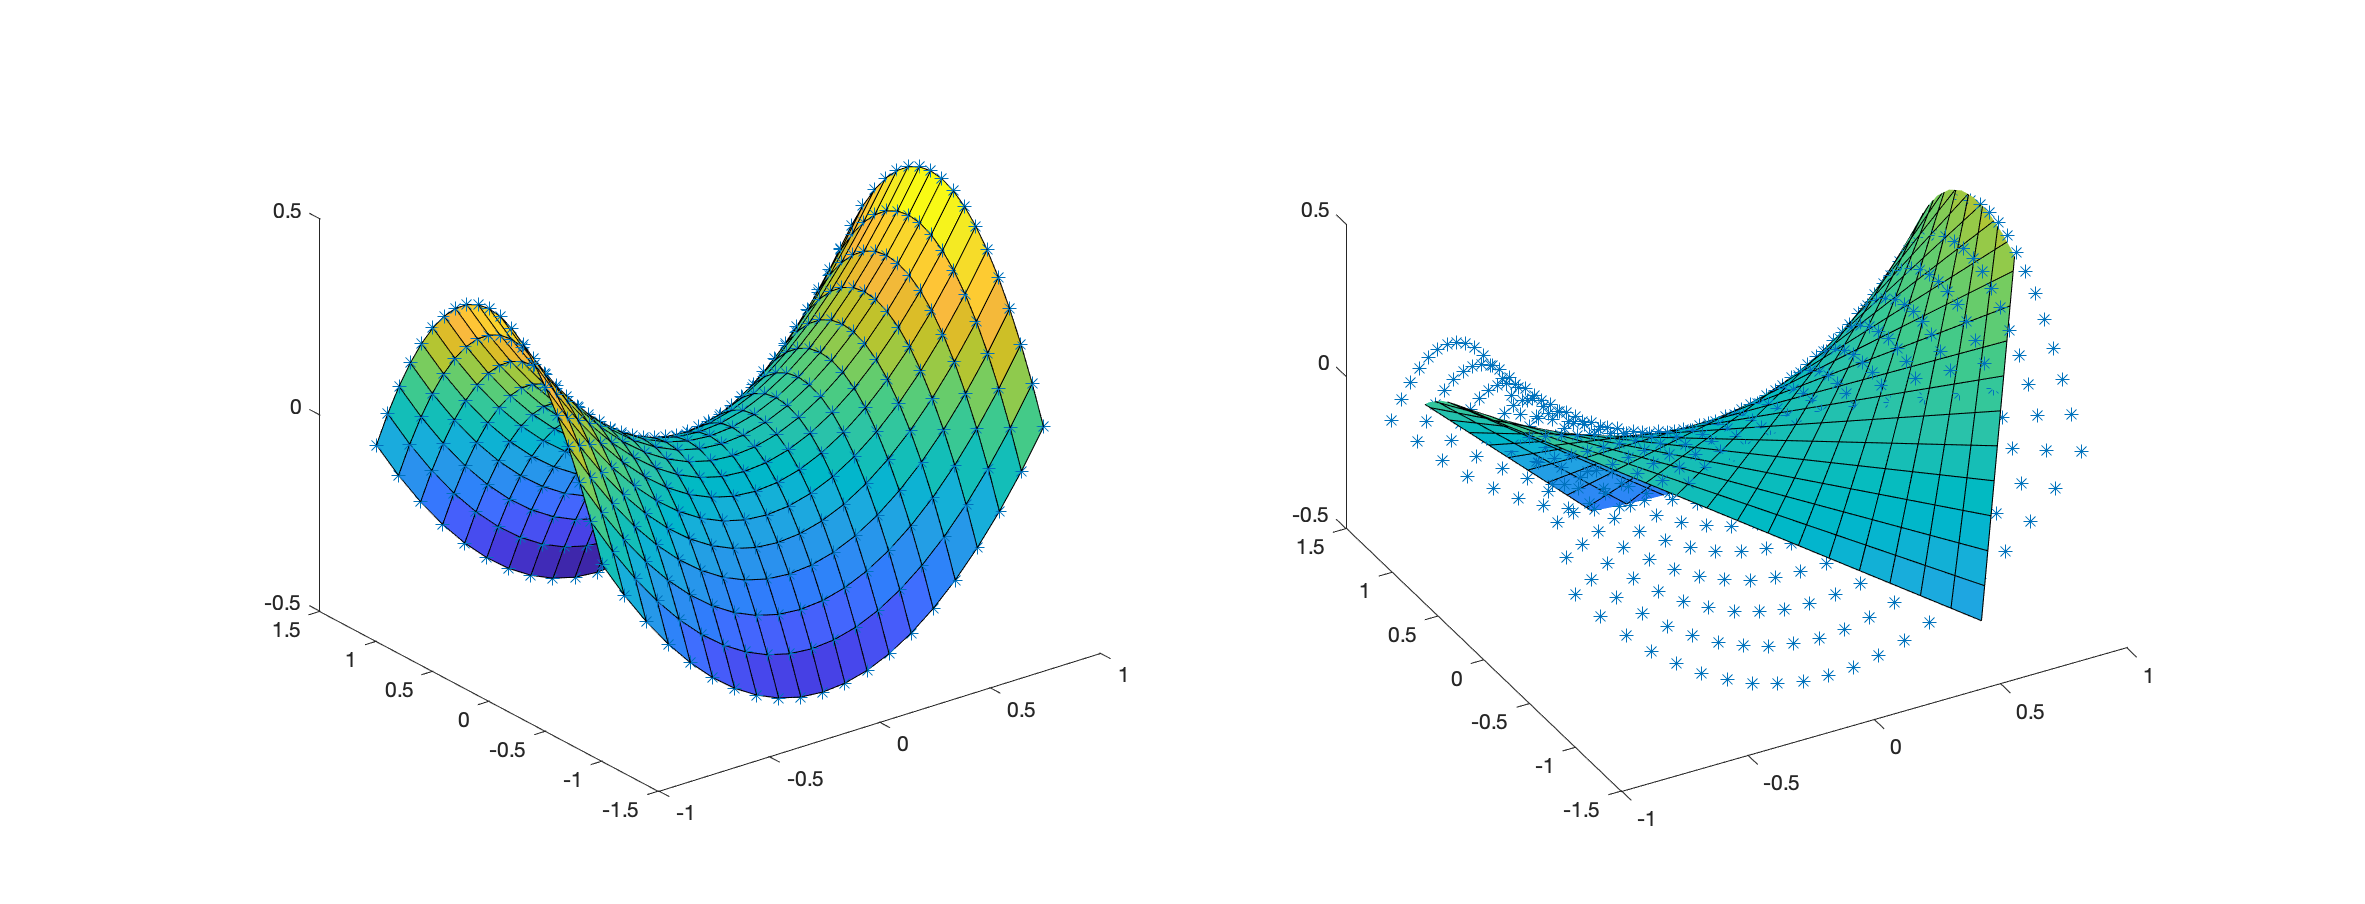
\includegraphics[width=\linewidth]{saddle.eps} 
%   \caption{Illustration of hyperbolic  fitting case: Left: fitting at $(0,0,0)$, Right: fitting at $(1/2,1/2,0)$. Data drawn from function $(x,y,z) = (\tau_1,\tau_2, {\tau_1^2}/{2}-{\tau_2^2}/{2})$ without distrurbed by noise:  }
%   \label{fig:example}
%\end{figure}
% 
% For general case in higher dimension,  an indefinite matrix $S^k$ will result in a  hyperbolic paraboloid in the corresponding dimension $k$ in normal space. Suppose $S^k$ yields a eigen-decomposition of the form
% \[
% S^k = [V_1,V_2]
% \left[
% \begin{array}{cc}
% \Lambda_1&0\\
% 0&\Lambda_2
% \end{array}
% \right]
% [V_1,V_2]^T,
% \]
% where the diagonal elements  of $\Lambda_1$ are positive, and diagonal ones of $\Lambda_2$ are negative. Thus, we know the space spanned by the columns of $U_\perp V_1$ is second order positive, i.e., any direction restricted in this space is a subspace-restricted local minimum point. Conversely,  the space spanned by the columns of $U_\perp V_2$ is second order negative, i.e., any direction restricted in this space is a subspace-restricted local maximum point. Thus, recalling that the second order surface is tangent to the first-order plane $\{x(\tau) |x(\tau)=x_0+U\tau\}$ at $x=x_0$, the origin point $x_0$ is a saddle point.
% 
% In our manifold fitting problem, because we do not has any prior information on the manifold besides the observations, we do not restrict $S^k$ to be a positive (or negative) matrix. The definite (or indefinite) property is decided by our fitting model and the inputed data.

%In this case, we have multiple choice of $S_k$ given the current observations. Any of the $S_k$ is the optimal solution for the 2-order fitting problem.
%\subsection{Solution}
%Depending on difference of the shape and the rank of $G$, we have the following cases:
%\subsubsection*{Case \romannumeral1: $m=\frac{d(d+1)}{2}$, ${\rm rank}(G) = \frac{d(d+1)}{2}$}
%In this case, \eqref{g_i} can be written as
%\[
%G  (vec({\rm Triu}(S^k))) = \ell_k
%\]
%Thus, $G$ is invertible, the closed-form of $vec({\rm Triu}(S^k))$ can be written as
%\[
%vec({\rm Triu}(S^k))  = {G}^{-1} \ell^k
%\]
%\remark{ Here, we can build $\psi(\tau)$ to go through all the $\frac{d(d+1)}{2}$ samples.
%}
%\subsubsection*{Case \romannumeral2: $m>\frac{d(d+1)}{2}$, ${\rm rank}(G) > \frac{d(d+1)}{2}$}
%
%\remark{ There are $d\times d$ parameters in $S^{k}$
%}
%\subsection{Asymptotic Properties}
%In this section, we give the asymptotic properties of our fitted $\hat{S}^k$ and the true $S^k$ (Hessian of $\phi_k(\tau)$ at $0$) with the behaviors of $n$ and $h$.
%\begin{theorem}
%For the estimated $\hat{\theta}_k$, the error between $\hat{\theta}_k$ and the true $\theta_k$ is with the order of 
%\[
%\hat{\theta}_k - \theta_k = O(h) +O_p(\frac{1}{\sqrt{nh^{D-2}}}),
%\] 
%where $n$ is the number of observations and $h$ is the bandwidth selected in our locally least square problem.
%\end{theorem}
%\begin{remark}
%Obviously, the optimum order of $h$ is $h=O(\frac{1}{n^{1/D}})$.  With the increasing of observations, we could choose a relatively small $h$ such that the estimated error is relatively small.
%\end{remark}

\section{Manifold Fitting via Nonlinear Projection}
In the former section, we show how to obtain the parameterized manifold $x_{\cal A}$ by taking the second order term $\cal A$ into consideration via the linear least square problem. In this section, we show how to implement a nonlinear projection onto our fitted manifold. %Meanwhile, we also give some theoretical results to ensure the convergence properties.
The manifold fitting problem can be viewed as projecting data $x$ onto a locally approximated structure. The existing manifold fitting methods all consider this local structure as a linear affine plane (parameter with $\tau$), such as
\[
 x(\tau)  =  U \tau +x_0.
\]

\begin{figure}[h] %  figure placement: here, top, bottom, or page
   \centering
   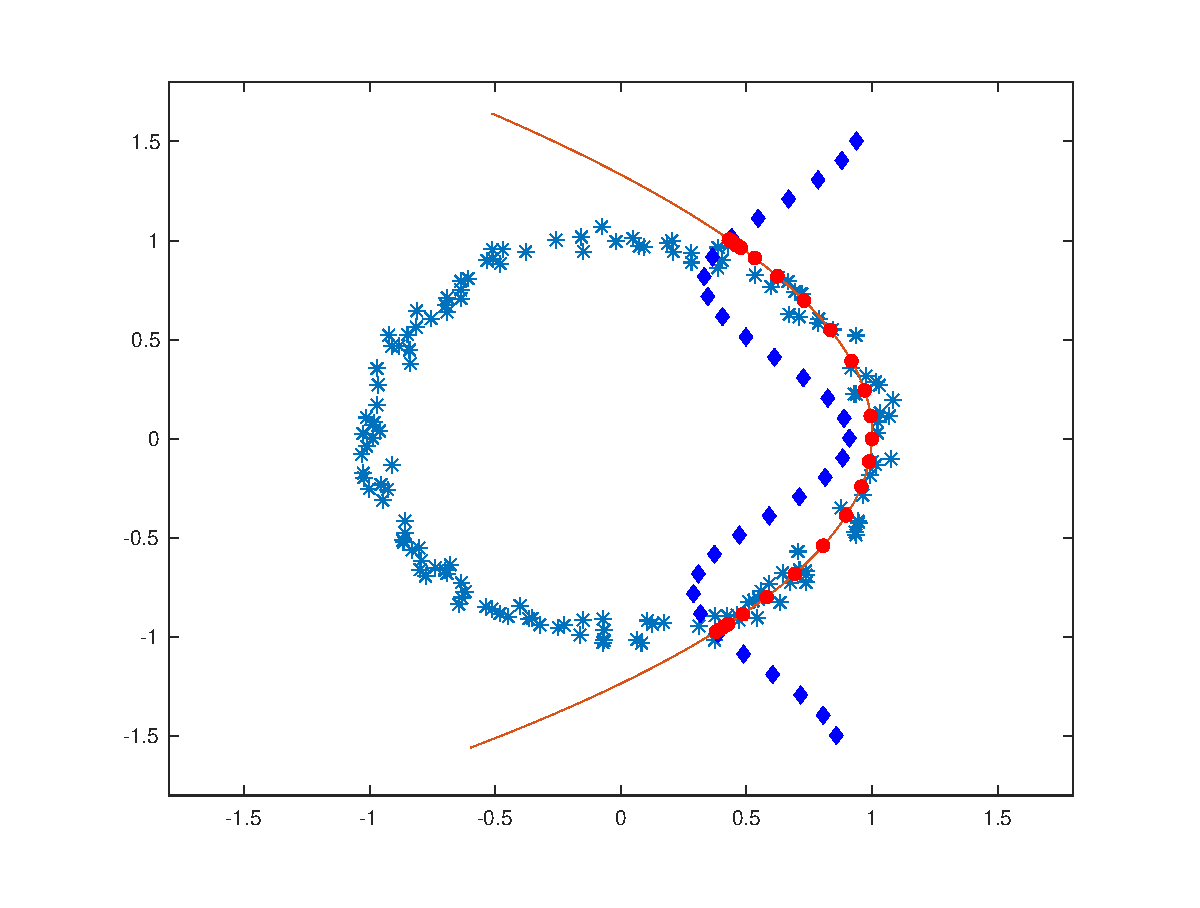
\includegraphics[width=0.8\linewidth]{demo3.eps} 
   %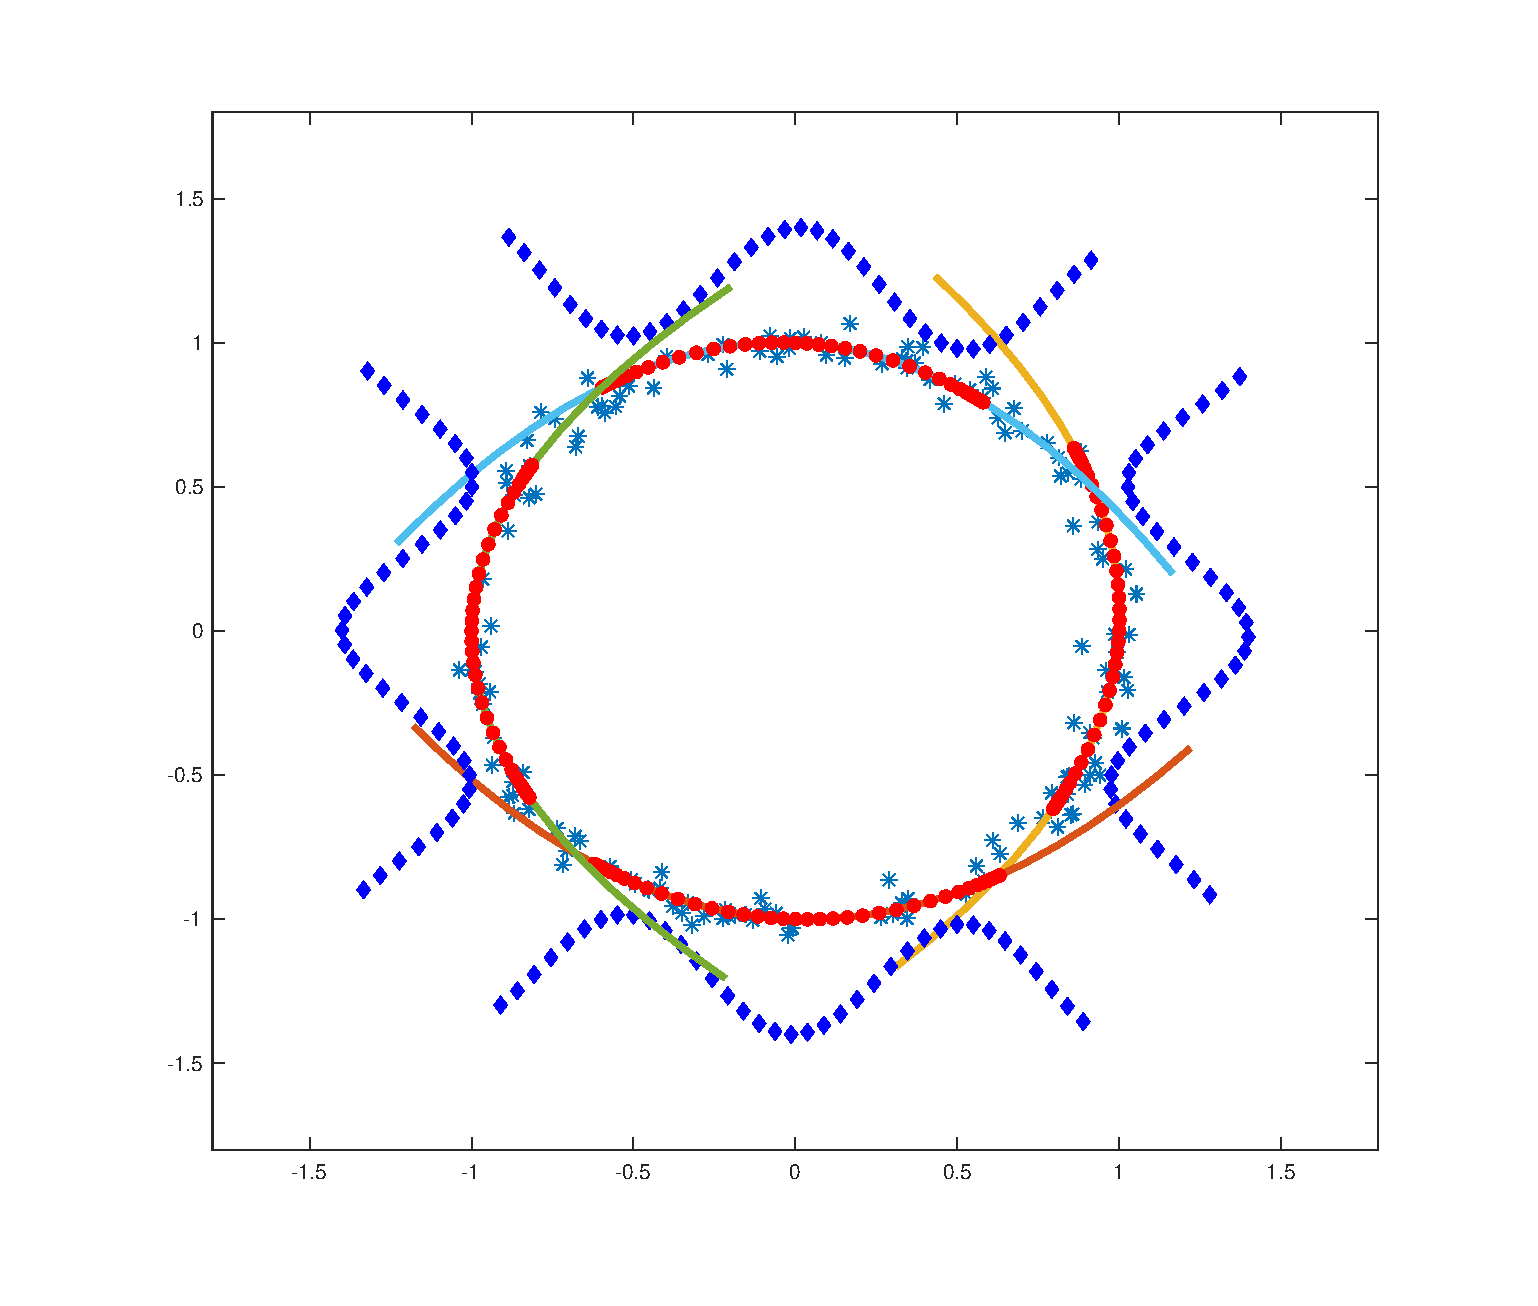
\includegraphics[width=0.48\linewidth]{fit_demo.eps} 
   \vspace{-0.4cm}
   \caption{Demo for the projection via solving the nonlinear least problem. The blue stars `*' are the discrete samples which are assumed to be approximately sampled from some manifold. The paraboloid curve is our fitted manifold with the second order term taken into consideration. The blue diamonds `$\diamond$' are the outliers, which can be any type or distribution. In this demo, we let the outliers to be samples from the $\sin$ curve. The red dots `$\circ$' are the projections of `$\diamond$' onto the paraboloid curve (the fitted manifold). In this section, we give the algorithm to find the projection of outliers onto the fitted second order function.}
   \label{fig:demo}
\end{figure}

%We give a demo in Figure \ref{fig:demo} to show our intuition. 


Different fitting approaches differ in the construction of $U$ and $x_0$.
In our work, we can have a fitted paraboloid (quadratic) surface, with the form as
\begin{equation}\label{manifold_representation}
x_{\cal A}(\tau) = U_{\perp} {\cal A} (\tau,\tau) + U \tau +x_0,
\end{equation}
where $x_0$ is the origin (center for the local coordinate) and ${\cal A} (\tau,\tau)$ represents the second fundamental form which is curvature function mapping from the tangent space to the normal space. 

\subsection{Projection onto Manifold}
Suppose we have a locally fitted manifold which has the parameterized form written as $x(\tau): {\mathbb R}^d\rightarrow {\mathbb R}^D$.
Since the range of the function $x_{\cal A}(\tau)$ generates a paraboloid manifold, we denote it as 
\[
{\cal M}_{\cal A} = \{y: y = x_{\cal A}(\tau), \tau\in {\mathbb R}^d\}.
\]
Given any $z\not\in{\cal M}_{\cal A}$, we define the projection $P_{{\cal M}_{\cal A}}(z)$  of $z$ onto ${\cal M}_{\cal A}$ as
\begin{equation}\label{projection}
P_{{\cal M}_{\cal A}}(z) = \arg\min_{w \in {\cal M}_{\cal A} }\|w-z\|_2.
\end{equation}
Using the function $x_{\cal A}(\tau)$, we know the points on ${\cal M}_{\cal A}$ and the Euclidean space $R^d$ is one-to-one. As a result, instead of find $w$, in \eqref{projection}, we just need to find $\tau$
\begin{equation}\label{projection_tau}
 \hat{\tau} = \arg\min_{\tau\in R^d }\|z-x_{\cal A}(\tau)\|_2^2.
\end{equation}
Finally, using the explicit form $x_{\cal A}(\tau)$, we know the projection yields
\[
P_{{\cal M}_{\cal A}}(z) = x_{\cal A}(\hat{\tau})=x(\arg\min_{\tau\in R^d }\|z-x_{\cal A}(\tau)\|_2^2).
\]
%\remark{ 
%In \eqref{projection_tau}, we minimize the squared of 2-norm instead of 2-norm for two reasons. First, optimizing with respect to $f^2(\cdot)=\|\cdot\|_2^2$ and $f(\cdot)=\|\cdot\|_2$ is equivalent because  $f^2(x)$ and $f(x)$ share the same monotonous property in the intervals of $\{x|f(x)>0\}$. Second, $\|\cdot\|_2^2$ is a polynomial, which has easier form with respect to derivatives for any order.
%}
Overall, the projection onto ${\cal M}_{\cal A}$ consists of the following two steps:
%\begin{itemize}

1. Solve the nonlinear problem: Given $z$, find $\tau$ such as 
\begin{equation}\label{nonlinear_projection}
\hat{\tau} = \min_\tau \|z -  (U_{\perp} {\cal A} (\tau,\tau) + U \tau +x_0)\|_2^2.
\end{equation}

2. Construct the coordinate in the ambient space
\[
\hat{z} = U_{\perp} {\cal A} (\hat{\tau},\hat{\tau}) + U \hat{\tau} +x_0.
\]
%\end{itemize}
To solve the nonlinear projection problem \eqref{nonlinear_projection}, we can simplify it as
\begin{equation}\label{simiplified_nonlinear}
\begin{aligned}
   &\|z -  (U_{\perp} {\cal A} (\tau,\tau) + U \tau +x_0)\|_2^2\\
 =&\|P_U(z-x_0)-U\tau\|_2^2+\|P_{U_{\perp}}(z-x_0)-(U_{\perp} {\cal A}(\tau,\tau))\|_2^2 \\
  =&\|U (U^T (z-x_0)-\tau)\|_2^2+\|U_\perp (U_{\perp}^T(z-x_0)- {\cal A}(\tau,\tau))\|_2^2 \\
 =&\|U^T (z-x_0)-\tau\|_2^2+\|U^T_{\perp}(z-x_0)- {\cal A} (\tau,\tau)\|_2^2.
\end{aligned}
\end{equation}

The optimization problem in \eqref{simiplified_nonlinear} is nonlinear, with the highest order term corresponding to $\tau$ is quartic. As far as we know, there is no closed-form solution to directly minimize \eqref{simiplified_nonlinear}. The difficulty originates from the relatively higher order. If we can decrease the order with respect to $\tau$ to 2, we will have a closed form. In next section, we show how to obtain the optimum $\tau$ via solving a series of quartic optimization problems.
\subsection{Quadratic Approximation}
In this section, we solve the quartic optimization problem by repeatedly implementing the quadratic approximation.
Firstly, for notational convenience, let's denote 
\[
s = U^T (z-x_0)\in {\mathbb R}^{d}, \quad c = U^T_{\perp}(z-x_0)\in {\mathbb R}^{D-d},
\]
where the bases $U^T$ and $U^T_{\perp}$ can be obtained from solving the locally principal component analysis problem (LPCA) centered at $x_0$. Consequently, $s, c$ can be obtained from $U^T$, $U^T_\perp$ and $x_0$.
%where $s, c$ can be obtained from solving the locally principal component analysis (PCA) centered at $x_0$. 
With these notations, the problem of \eqref{simiplified_nonlinear} can be converted into:
\begin{equation}\label{f_tau}
f(\tau) = \|s-\tau\|_2^2+\|c- {{\cal A}} (\tau,\tau)\|_2^2.
\end{equation}
Note that, ${{\cal A}} (\tau,\tau)$ is the quadratic form with respect to $\tau$ and $\|c- {{\cal A}} (\tau,\tau)\|_2^2$ is the quartic term. Even though $f(\tau)$ is a polynomial function with the input as a vector $\tau$, it is still difficult to obtain the closed form for $\tau$. Based on this observation, we reduce the order of $f(\tau)$ 
by bringing in the auxiliary function $g(\tau_1,\tau_2)$, which is defined as
\[
g(\tau_1,\tau_2) =\frac{1}{2} \|s-\tau_1\|_2^2+\frac{1}{2} \|s-\tau_2\|_2^2+\|c- {\cal A} (\tau_1,\tau_2)\|_2^2.
\]
Because of the symmetric property of $g(\tau_1,\tau_2)$ with respect to $\tau_1$ and $\tau_2$, we have
\[
g(\tau_1,\tau_2) = g(\tau_2,\tau_1).
\]
When fixing $\tau_1$, the quadratic function $g(\tau_1,\tau)$ approximates $f(\tau)$ with a small error when $\tau$ approaches $ \tau_1$. For the extreme case, when $\tau=\tau_1$, we have $g(\tau_1,\tau_1)=f(\tau_1)$. By minimizing via alternating fixing $\tau_1$ and $\tau_2$, we could derive a sequence of $\{\tau_n, n=1,2...,\}$ in \eqref{min_tau_n} by
%\[
%\tau_{n+1} = \min_\tau g(\tau_n,\tau)
%\]
%\[
%\min_\tau f(\tau) \geq \min_{\tau_1,\tau_2} g(\tau_1,\tau_2)
%\]
%Fix $\tau_2$, minimize $g(\tau_1,\tau_2)$ with respect to $\tau_1$ is a least square problem
\begin{equation}\label{min_tau_n}
\begin{aligned}
&\tau_{n+1} = \arg\min_{\tau} g(\tau_{n},\tau)  \\
=&\arg\min_{\tau}\frac{1}{2}\|s-\tau_{n}\|_2^2+\frac{1}{2}\|s-\tau\|_2^2+\|c-{\cal A}(\tau_{n})\tau\|_2^2.
\end{aligned}
\end{equation}
For notational convenience, define $\phi(\tau_{n})$ as the optimal minimum solution of \eqref{min_tau_n}, i.e,
\[
\phi(\tau_{n})=( 2{\cal A}(\tau_{n}){\cal A}(\tau_{n})^T+ I_d)^{-1} (2{\cal A}(\tau_{n})c+ s).
\]
%Next, we give the Theorem \ref{global} by showing that $\phi(\tau_n)$ is the global minimal point for the quadratic function $g(\tau_n,\tau)$ with respect to $\tau$.
%\begin{theorem}\label{global}
%The global minimal point of  $g(\tau_{n},\tau)$ is $\tau = \phi(\tau_{n})$.
%\end{theorem}
%\begin{proof}
%Taking the derivative of $g(\tau_n,\tau)$ with respect to $\tau$, we get the gradient $\nabla_\tau g(\tau_n, \tau)$ as %$\nabla_\tau g(\tau_n, \tau)=0$ for $\tau$ leads to
%\[
%\nabla_\tau g(\tau_n, \tau) = 2({\cal A}(\tau_n){\cal A}(\tau_n,\tau)-{\cal A}(\tau_n)c) +(\tau-s).
%\]
%Let $\nabla_\tau g(\tau_n, \tau)=0$ and solve the linear equation $\nabla_\tau g(\tau_n, \tau)=0$  with respect to $\tau$, we obtain the closed-form of $\tau$ as 
%\[
%\tau = ( 2{\cal A}(\tau_{n}){\cal A}(\tau_{n})^T+ I_d)^{-1} (2{\cal A}(\tau_{n})c+ s).
%\]
%%Denote $\phi(\tau_{n})$ as
%%\[
%% \phi(\tau_{n})=( 2{\cal A}(\tau_{n}){\cal A}(\tau_{n})^T+ I_d)^{-1} (2{\cal A}(\tau_{n})c+ s).
%%\]
%Since the optimal property is highly related with the second-order differential forms, taking the second-order differential operation in $g(\tau_n, \tau) $ with respect to $\tau$, we obtain the Hessian $H_g(\tau)$ as 
%\[
%H_g(\tau) = \nabla_\tau \nabla_\tau g(\tau_n,\tau) = 2{\cal A}(\tau_n){\cal A}^T(\tau_n)+I_d.
%\]
%Because ${\cal A}(\tau_n){\cal A}^T(\tau_n)$ is a $d\times d$ semi-positive definite matrix and $I_d$ is the identity which is positive definite, we know $H_g(\tau)$ is a constant positive definite matrix which does not rely on $\tau$, which implies that $\tau = \phi(\tau_{n})$ is the global minimal point of $g(\tau_n,\tau)$. 
%%Therefore, $\phi(\tau_{n})$ has a closed-form to be $\hat{\tau}(\tau_n)$, i.e.,
%%\[
%% \phi(\tau_{n})=( 2{\cal A}(\tau_{n}){\cal A}(\tau_{n})^T+ I_d)^{-1} (2{\cal A}(\tau_{n})c+ s).
%%\]
%\end{proof}
%\[
%g(\tau_{n},\tau_{n+1}) \leq g(\tau_{n},\tau_{n})
%\]
Using $\phi(\tau_n)$, we can define a vector sequence $\{\tau_n, n = 1,2...,\}$ via the fixed-point iteration by
$\tau_{n+1} = \phi(\tau_n)$
and set the convergence point $\tau^*$ as the coordinate for the true projection.
%Next, we give the convergence property of the sequence $\{\tau_n, n = 1,2...,\}$.
%\begin{theorem}\label{convergence}
%%For the auxiliary function value of $g(\tau,\beta)$, 
%The sequence $\{a_n = g(\tau_n,\tau_n+1), n=1,2...,\infty\}$ is monotonously decreasing with a positive lower-bound, thus it is a convergent sequence!  
%%Where the vector sequence $\{\tau_n, n = 1,2...,\}$  is generated from the fixed point iteration 
%%\[
%%\tau_{n+1} = \phi(\tau_n),
%%\]
%%satisfies the value sequence of the auxiliary function, $\{g(\tau_n,\tau_n+1)\}$ 
%\end{theorem}
%\begin{proof}
%Using the symmetric property of function $g$, we have:
%\begin{equation}\label{relation1}
%g(\tau_{n},\tau_{n-1})= g(\tau_{n-1},\tau_n).
%\end{equation}
% Meanwhile, because of the optimal minimizing relation $\tau_{n+1}=\arg\min g(\tau_{n},\tau)$, we know
% \begin{equation}\label{relation2}
% g(\tau_{n},\tau_{n+1}) \leq  g(\tau_{n},\tau_{n-1}).
% \end{equation}
%Combining the above two relations in \eqref{relation1}\eqref{relation2}, we have:
%\[
%g(\tau_{n},\tau_{n+1}) \leq g(\tau_{n},\tau_{n-1})= g(\tau_{n-1},\tau_n). %\leq g(\tau_{n-1},\tau_{n-1})
%\]
%Therefore, the sequence $\{g(\tau_{n},\tau_{n+1})\}$ decreases with $n$. Also $\{g(\tau_{n},\tau_{n+1})\}$ has a lower bound because it is positive. Using the monotonous-bound theorem, we know the sequence $\{g(\tau_{n},\tau_{n+1})\}$ converges!
%\end{proof}
%From \eqref{min_tau_n}, we know
%\[
%\nabla g(\tau_n,\tau_{n+1}) = 0,\quad \lambda_k (H_g(\tau_{n+1})) \geq 0,
%\]
%which is equivalent to 
%\[
%2({\cal A}(\tau_n){\cal A}(\tau_n,\tau_{n+1})-{\cal A}(\tau_n)c) +(\tau_{n+1}-s)= 0.
%\]
%Because the sequence $\{g(\tau_n,\tau_{n+1})\}$ converges, denote the unique limit of the sequence as
%\[
%\gamma = \lim_{n\rightarrow \infty} g(\tau_n,\tau_{n+1}).
%\]
%Next, we will show, under some conditions, $\gamma$ is also the minimum of $f(\tau)$. This result relies on the convergence property of the vector sequence $\{\tau_n,n=1,...,\infty\}$. As the sequence of $\tau_n$ is generated from the fixed point iteration, to guarantee the convergence, we can give a stricker condition by requiring $\phi(\tau)$ to be a contraction map.
%
%Similarly with the matrix, define the norm of the tensor as 
%\[{
%\|{\cal A}\|_2 = \max_{\|c\|=1}\|{\cal A}(c)\|_2=\max_{\|c\|=1,\|\tau\|=1} \cal A}(\tau,\tau,c).
%%\max_{\tau\neq 0,c\neq 0} \frac{\sum_{ijk}{\cal A}_{ijk}\tau_i \tau_j c_k}{\|\tau\|_2^2 \|c\|_2} = \max_{\|c\|_2=1} \|\sum_k {\cal A}_{\cdot\cdot k}c_k\|_2.
%\]
%%\subsection{Contraction Map and Optimal}
%%Define $\phi(\tau_{n}) = \arg\min_\tau g(\tau_n,\tau)$. Because $g(\tau_n,\tau)$ is quadratic form with respect to $\tau$, $g(\tau_n,\tau)$ has a unique global minimizer. Taking the derivative with respect to $\tau$, we have
%%\[
%%\nabla_\tau g(\tau_n, \tau) = 2({\cal A}(\tau_n){\cal A}(\tau_n,\tau)-{\cal A}(\tau_n)c) +(\tau-s).
%%\]
%%Next, we show that $\phi(\tau_{n})$ to be a contraction map. 
%
%\begin{theorem}\label{contraction}
%If $L = (4\beta^2\|{\cal A}\|_2^3\|c\|_2+2\|s\|_2\|{\cal A}\|_2^2)<1$,  then, the function $\phi(\tau)$ is a contraction map, i.e,
% \[
% \|\phi(\tau_{n-1})- \phi(\tau_{n})\|_2 \leq L\|\tau_{n-1} -\tau_n \|_2,
% \]
%where $\beta$ is the upper bound of $\|\tau_n\|_2$, i.e., $\beta = \sup_n\|\tau_n\|_2$.
%\end{theorem}
%The proof is left in the appendix \ref{contraction}. Recall that $s = U^T (z-x_0)\in {\mathbb R}^{d}$ is the local coordinate of $z$ in the tangent space.  $c = U^T_{\perp}(z-x_0)\in {\mathbb R}^{D-d}$ is the coordinate in the normal space. When selecting a good origin $x_0$, we can have the norm of $s$ and $c$ to be in small scale simultaneously, so as to make $L$ as small as possible.
%\begin{remark}
%$\|{\cal A}\|_2$ represents the maximum curvature of underlining manifold which can be obtained through solving the fitting model from the observations. It can be seen that if the manifold becomes more and more flatter, $L$ will turn more smaller which will makes the requirement of our assumption easily to be satisfied.
%\end{remark}
%
%The contraction mapping theorem shows that, for a complete metric space, if $\phi(\tau)$ is a contraction, $\{\tau_n, n=1,2,...\}$ is a Cauchy sequence. Furthermore, it converges to a unique fixed point $\tau^*$. Theorem \ref{contraction} is the sufficient but not necessary condition for $\{\tau_n, n=1,2,...\}$ to be the convergent sequence.
%
%\begin{theorem}
%The convergence point $\tau^*$ of $\{\tau_n, n=1,2....\}$ is a stationary point of $f(\tau)$. Furthermore, if 
%\[
%I_d+2{\cal A}({\cal A}(\tau^*,\tau^*)-c) + 4{\cal A}(\tau^*){\cal A}^T(\tau^*),
%\] 
%is positive definite, $\tau^*$ is also an optimal minimal of $f(\tau)$.
%\end{theorem}
%\begin{proof}
%Since $\{\tau_n, n=1,2...\}$ is a Cauchy sequence, taking the limit of $n$ leads to
%\[
%\lim_{n\rightarrow\infty} g(\tau_n,\tau_{n-1}) = g(\tau^*,\tau^*) = f(\tau^*).
%\]
%From the optimal of $\tau_{n+1}=\min_{\tau} g(\tau_n,\tau)$, we have $\nabla_{\tau} g(\tau_n,\tau)|_{\tau=\tau_{n+1}}=0$, i.e.,
%\begin{equation}\label{optimal_g}
%2({\cal A}(\tau_n){\cal A}(\tau_n,\tau_{n+1})-{\cal A}(\tau_n)c) +(\tau_{n+1}-s)= 0.
%\end{equation}
%In \eqref{optimal_g}, taking the limit with respect to $n$, we have $\tau^*=\lim \tau_n$ which satisfying the normal equation as
%\begin{equation}\label{normal}
%2({\cal A}(\tau^*){\cal A}(\tau^*,\tau^*)-{\cal A}(\tau^*)c) +(\tau^*-s)= 0.
%\end{equation}
%Recall that $\nabla f(\tau) = 2(\tau-s)+4({\cal A}(\tau,\tau)-c) {\cal A}(\tau)$.
%Obviously, we know $\tau^*$ also satisfies the KKT condition for $f(\tau)$, i.e.,
%$\nabla f(\tau^*) = 0$.  Thus, $\tau^*$ is a stationary point $f(\tau)$. Next, to check $\tau^*$ is a local minimum, we need to check the definite property of the second-order derivatives, $H_f(\tau)$,
%\[
%H_f(\tau) = 2I_d+4{\cal A}({\cal A}(\tau,\tau)-c) + 8{\cal A}(\tau){\cal A}^T(\tau).
%\]
%Clearly, $\tau^*$ is an optimal minimum of $f(\tau)$ if and only if $H_f(\tau^*) $ is a positive definite matrix. 
%
%Note that, ${\cal A}(\tau,\tau)-c\in {\mathbb R}^{D-d}$, the tensor $\cal A$ acting on the $D-d$ dimensional vector ${\cal A}(\tau,\tau)-c$ is the reduce-sum operation along the third dimension of $\cal A$, which will result in a symmetric matrix.
%\end{proof}
%\begin{figure}[h] %  figure placement: here, top, bottom, or page
%   \centering
%   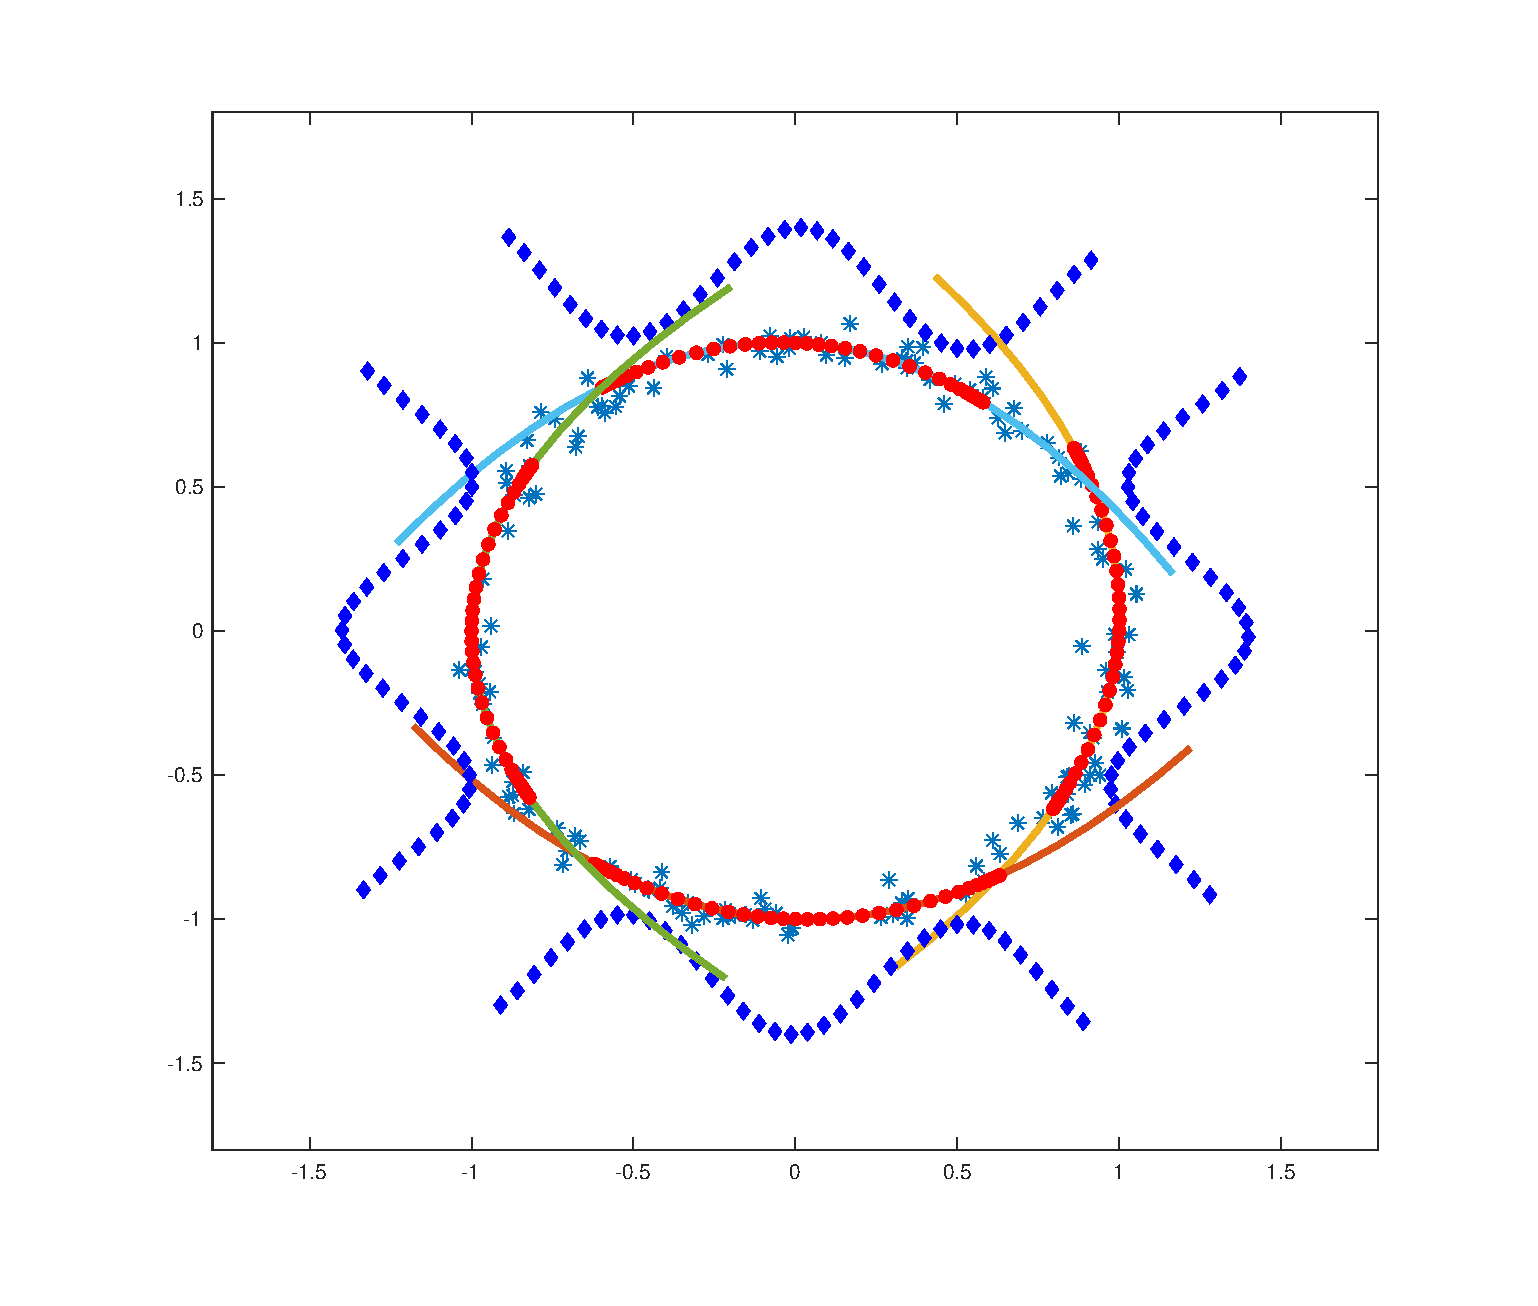
\includegraphics[width=\linewidth]{fit_demo.eps} 
%   \caption{Projecting the outlier points onto the fitted manifold}
%   \label{fig:section_example}
%\end{figure}
%In Figure \ref{fig:section_example}, we give a demo by dividing the samples into four partitions as the four $\sin$ curve sets. The projections of the blue `$\diamond$' points are marked as the red `$\circ$' dots which can be regarded as the approximation of the projection onto the real underlying manifold. It is obviously shown from Figure \ref{fig:section_example} that projecting by fitting locally is a good approach to handle the difficult manifold fitting problem. Furthermore, we can fit a locally quadratic manifold for each of the outliers which we want to pull back onto $\cal M$. The details can be seen from the description in the algorithm in section \ref{nonliear projection}.
%Denote $N(x_{\ell}(\tau), {\cal M}, \epsilon )$ and $N(x_{\cal A}(\tau), {\cal M}, \epsilon )$ as the numbers of ${\cal M}_\ell$ and $\cal M_{\cal A}$ to cover the underlying manifold $\cal M$ with the maximum fitting error $\epsilon$. Denote ${\cal M}_{\ell}(x_0)$ and ${\cal M}_{\cal A}(x_0)$ as the fitting manifolds which are the range of functions $x_\ell(\tau)$ and $x_{\cal A}(\tau)$ respectively and goes through $x_0$. We have the following theorem:
%\begin{theorem}
%Under the fitting error tolerance setting as $\epsilon$, the ratio for the numbers of the fitting structure needed to cover $\cal M$ by $x_{\ell}(\tau)$ and $x_{\cal A}(\tau)$ yields
%\[
%\frac{N(x_{\ell}(\tau), {\cal M}, \epsilon )}{N(x_{\cal A}(\tau), {\cal M}, \epsilon )}=O(\epsilon^{-d/6}).
%\]
%\end{theorem}
%\begin{proof}
%Define 
%$
%{\cal M}(x_0,\delta) = \{x| x \in {\cal M},d(x, x_0) \leq \delta\}.
%%???\{x| x \in {\cal M},d(x, {\cal \hat{M}}(x(\tau), x_0)) \leq \delta\}
%$, For $x\in {\cal M}\cap {\cal D}_{x_0}(\delta)$, we know:
%\[
%d(x, {\cal M_A}(x_0)) = O(\|\tau\|_2^3).
%\]
%Similarly, for the linear fitting function $x_\ell(\tau) = U_d\tau+x_0$ of $\cal M$, we have the projection error yielding:
%\[
%d(x, {\cal {M}}_\ell(x_0)) = O(\|\tau\|_2^2),
%\]
%where $\tau=U_d^T(x-x_0)$ which is the local coordinate of $x$. If we set the maximum tolerance to be 
%\begin{equation}\label{error_res}
%d(x, {\cal M_ A}(x_0))\leq \epsilon,\quad d(x, {\cal M}_\ell (x_0)) \leq \epsilon.
%\end{equation}
%From \ref{error_res}, we know the maximum radii for $\tau$ are of order $\epsilon^{1/3}$ and $\epsilon^{1/2}$ for $x_{\cal A}(\tau)$ and $x_{\ell }(\tau)$,  respectively.
%For the d-dimensional manifold, the volume for the ball with radius corresponding $\epsilon^{1/3}$ and $\epsilon^{1/2}$ are
%\[
%\begin{aligned}
%&{\rm Vol} \{x| x\in {\cal M},d(x, {\cal M}_{\ell}(x_0))\leq \epsilon \} =O( \epsilon^{d/2})\\
%&{\rm Vol} \{x| x\in{\cal M}, d(x, {\cal M_ A}(x_0))\leq \epsilon \} =O(\epsilon^{d/3}).
%\end{aligned}
%\]
%As a consequence, the numbers of the fitting structures needed to cover $\cal M$ with error $\epsilon$ are of $O( \epsilon^{-d/2})$ and $O(\epsilon^{-d/3})$ for $x_{\cal \ell}(\tau)$ and $x_{\cal A}(\tau)$, respectively. Obviously, the ratio is  $O(\epsilon^{-d/3})/O( \epsilon^{-d/2}) = O( \epsilon^{d/6})$.
%\end{proof}
%
%Next, we give a theorem to show that the minimal distance in the Euclidean space and the orthogonal properties are equivalent. That is to say, if we can find some point $x^*$ on ${\cal M_A}$ which is nearest from $x$, then $x-x^*$ is orthogonal with the tangent plane $ {\cal T}_{\cal M_A} (\tau^*)$ of $\cal M_A$ at $x^*$.
%\begin{theorem}
%For any $x$, denote the projection of $x$ onto ${\cal M_A}$ as $x^*$ and correspondingly there is the local coordinate $\tau^*$ such that $x(\tau^*)=x^* $, then we have
%\[
%x-x^* \perp {\cal T}_{\cal M_A} (\tau^*).
%\]
%\end{theorem}
%\begin{proof}
%Recalling that $x_{\cal A}(\tau) = U_\perp {\cal A}(\tau,\tau)+U(\tau)+x_0$, the tangent space ${\cal S}^*$ at $x_{\cal A}(\tau)|_{\tau^*}$ is spanned by the derivatives as
%\[
%{\cal S}^* = {\rm span}\{\nabla_{\tau_1} x_{\cal A}(\tau)|_{\tau=\tau^*}, \nabla_{\tau_2} x_{\cal A}(\tau)|_{\tau=\tau^*},...,\nabla_{\tau_d} x_{\cal A}(\tau)|_{\tau=\tau^*}\}.
%\]
%Note that, $\cal S^*$ is a subspace of  ${\mathbb R}^{D}$ and the basis of $\cal S^*$ consists of the columns of the Jacobi matrix  $J(x_{\cal A}(\tau))|_{\tau^*}$.
%%which corresponding to each columns of the Jacobi matrix $J(x_{\cal A}(\tau))|_{\tau^*}$. 
%which has a closed form of $J(x_{\cal A}(\tau))|_{\tau^*}$ as
%\[
%J(x_{\cal A}(\tau))|_{\tau=\tau^*} = 2U_\perp {\cal A}(\tau^*) + U.
%\]
%$\cal S^*$ is also the space spanned by the columns of $J(x_{\cal A}(\tau))|_{\tau=\tau^*}$. To prove $x-x^* \perp {\cal T}_{\cal M_A}({x^*})$, we just need to prove $x-x^*$ is orthogonal with each of the columns of $J(x_{\cal A}(\tau))|_{\tau=\tau^*}$. Next, we give the particular form of $x-x^*$, recall that
%\[
%\begin{aligned}
%&x-x^*\\
% =& x -  (U_\perp {\cal A}(\tau^*,\tau^*)+U\tau^*+x_0)\\
%	=& U_\perp (U_\perp^T(x-x_0) - {\cal A}(\tau^*,\tau^*)) +U(U^T(x-x_0)-\tau^*)\\
%	=& U_\perp(c_x - {\cal A}(\tau^*,\tau^*))+U(s_x-\tau^*).
%\end{aligned}
%\]
%It is easy to verify
%\[
%\begin{aligned}
%&(x-x^*)^T J(x_{\cal A}(\tau))|_{\tau=\tau^*}\\
% =& -\{({\cal A}(\tau^*){\cal A}(\tau^*,\tau^*)-{\cal A}(\tau^*)c_x) +(\tau^*-s_x)\}\\
% =& 0,
%\end{aligned}
%\]
%where the last equality is obtained from the optimal condition in \eqref{normal}, that is to say, $x-x^*$ is orthogonal with the subspace $\cal S^*$.
%\end{proof}
%\section{Origin Point Selection} \label{Origin Point Selection}
%The selection of the origin point $x_0$ is important for our fitting. A good quality $x_0$ will make the approximation error much smaller. If our observations $\{x_i, i=1,...,n\}$ are drawn exactly from $\cal M$ (no noise contaminated), we can select $x_0$ to be the point which is nearest to $\bar{x}$.
%\[
%x_0 = \arg\min_{\{x_i\}} \|\bar{x}-x_i\|_2.
%\]
%Otherwise, if the observations $\{x_i, i=1,...,n\}$ are drawn from $\cal M$ with noise, we can select $x_0$ as the weighted-mean as:
%\begin{equation}\label{weighted_mean}
%x_0 =\frac{1}{\sum_{i\in {\cal N}_k(\bar{x}) } \phi_h(\bar{x},x_i)} \sum_{i\in {\cal N}_k (\bar{x})} \phi_h(\bar{x},x_i)x_i,
%\end{equation}
%where $\phi_h(\bar{x},x_i) = K_h(x_i, \bar{x})$ is the kernel weight and ${\cal N}_k$ controls the neighbor size and $h$ is the bandwidth parameter, which affect the bias and smoothness. If we further denote 
%\[
%w_h(\bar{x},x_i)=\phi_h( \bar{x},x_i) / (\sum_{i\in {\cal N}_k (\bar{x})} \phi_h(\bar{x},x_i)),
%\]
%the equation \eqref{weighted_mean} can be further simplified as a convex combination of samples $\{x_i, i=1,...,n\}$ in the neighborhood ${\cal N}_k(\bar{x})$ of $\bar{x}$ as $x_0 = \sum_{i\in {\cal N}_k (\bar{x})} w_h(\bar{x},x_i) x_i$.
%
%Even though $x_0$ is not on the underlying manifold $\cal M$, we can still use it as the origin for $x_{\cal A}$ to project $\bar{x}$.  If obtaining a parameterized manifold $\cal M_A$ to locally approximate $\cal M$, we can quantify the distance between the weighted-mean $x_0$ and $\cal M_A$. Since $\cal M_A$ locally fits $\cal M$, the distance between $x_0$ and $\cal M_A$ can be used in place of the distance between $x_0$ and $\cal M$ as long as the scale of the local coordinate $\tau$ is small enough.
%\begin{assumption}
%If the observations are drawn from the quadratic manifold, which can be parameterized in the form 
%$
%x_{\cal A}(\tau) = U \tau+ U_\perp {\cal A}(\tau, \tau)+x_0^*.
%$
%and the samples are generated as $\{x_i = U \tau_i + U_\perp {\cal A}(\tau_i,\tau_i)+x_0^* + \epsilon_i, i=1,...,m\}$, where $\{\tau_i,i=1,...,m\}$ can be drawn uniformly from a d-dimensional ball in the tangent space and the noise $\epsilon_i$ is the independent noise obeying some distribution, such that normal $\{\epsilon_i |\epsilon_i \sim {\cal N}(0, \sigma I)\}$ with $\sigma$ is the scale of the disturbed noise.
%\end{assumption}
%\begin{theorem}
%For any $x_0$ defined as a summation of point in \eqref{weighted_mean},  the Euclidean distance from $x_0$ to the manifold $\cal M_A$ is upper-bounded by
%\[
%\min_{y\in {\cal M_A}} d (x_0, y) \leq  \|{\cal A}\|_2O(h^2)+\sigma O_p(\sqrt{mD}).
%\]
%%\[
%%{\rm E} (\min_\tau \|x_0-x(\tau)\|_2^2) \leq {\rm E} (\|x_0-x(\tau_w)\|_2^2) \leq \max_k(\lambda_{k} ({{\cal A}_{\cdot,\cdot,k}})) O({r}^4h^4)+ {\sigma^2}
%%\]
%\end{theorem}
%The proof is left in the appendix \eqref{dis_x0}.
%\remark{
%The distance from $x_0$ to $\cal M_A$ is influenced by three factors $\cal A$, $h$ and $\sigma$. If the curvature tensor ${\cal A}$ approaches $\bf 0$, the fitted manifold $\cal M_A$ will become a flat plane gradually. Thus, any linear combination of samples from a affine space will also belong to the affine space. When $h$ approaches $0$, $x_0$ will become the nearest neighbor of $\bar{x}$, since the weight corresponding to the nearest neighbor will become dominant compared with the remaining points. Under the condition that $h$ approaches $0$, and $\sigma\rightarrow 0$, $x_0$ will approaches the nearest neighbor of $\bar{x}$ which also belongs to $\cal M_A$.
%
%%the distance $d(x_0,{\cal M_A})$ turns smaller when $x_0$ to $\cal M_A$.
%}
%
\section{Algorithm: Projection by Repeated Nonlinear Least Square}\label{nonlinear projection}
Because the underlying manifold is unknown, in real computational cases,  we cannot find a point $x_0\in \cal M$ which is also next to our interested outlier $\bar{x}$. To solve this problem, we use an iteration method to find $x_0$. When $\bar{x}$ is far away from $\cal M$, the inaccurate of $x_0$ is also acceptable. With the process of $\bar{x}$ approaching $\cal M$, we need the accuracy of  $x_0$ to be improved.
Since the observations $\{x_i, i=1,...,n\}$ are drawn from $\cal M$ with noise, for the outlier $\bar{x}$, we can select $x_0$ as the weighted-mean as:
\begin{equation}\label{weighted_mean}
x_0 =\frac{1}{\sum_{i\in {\cal N}_k(\bar{x}) } \phi_h(\bar{x},x_i)} \sum_{i\in {\cal N}_k (\bar{x})} \phi_h(\bar{x},x_i)x_i,
\end{equation}
where $\phi_h(\bar{x},x_i) = K_h(x_i, \bar{x})$ is the kernel weight and ${\cal N}_k$ controls the neighbor size and $h$ is the bandwidth parameter, which affect the bias and smoothness.

\begin{algorithm}[H]
\caption{Fitting Algorithm:}
\label{alg:Fitting}
\begin{algorithmic}
\STATE [1.] For outlier $\bar{x}$, compute the shift mean $x_0$ from \eqref{weighted_mean} and use $x_0$ as the origin of our local coordinate to implement our fitting and projection process.
\STATE [2.] Given $x_0$, neighborhood size $k$ and bandwidth parameters $h$, get the local coordinate $\{\tau_i, \iota_i\}$ for each $x_i$ by applying the eigen-decomposition method.
$
{\tau}_i = U_d^T(x_i-x_0).%,\quad \hat{\iota}_i = {{U^T_{n-d}}}(x_i-x_0)
$
Using $\tau_i$, construct matrix $G$ from $\{\tau_i\}$ such as $G = [g_1,...,g_m]^T$, where each column consists $g_i = {\rm vech}(\tau_i\tau_i^T, 1)$.% is the vectorization form.
\STATE [3.] Solve the manifold fitting problem for each dimension in the normal space, e.g, %solve the weighted least square problem in the $k$-th dimension of the normal space via minimizing:
for the $k$-th dimension:
\[
\begin{aligned}
  &\min_{\theta_k} \sum_{i=1}^m K_h(x_i-\bar{x})\{ g_i^T \theta_k  -  {(u^k_{x_0})}^T (x_i -x_0)/2\}^2\\
= &\min_{\theta_k}\|W_h^{1/2}(G \theta_k-\ell_k/2) \|_2^2,
\end{aligned}
\]
where the $m$ (number of samples in the neighborhood) dimensional vector $\ell_k$ equals to $[u_k^T(x_1-x_0), u_k^T(x_2-x_0),...,u_k^T(x_n-x_0)]$.
\STATE [4.] For each $k=1,...,D-d$, transform the vector $\theta_k$ into the matrix form by putting the elements of $\theta_k$ onto the upper-triangle positions to obtain ${\rm Mat}(\theta_k)$.  Afterwards, the symmetric $S_k$ is obtained via %of $M_k = {\rm Mat}(\theta_k)$:
$
S_k = {\rm Mat}(\theta_k) + {\rm Mat}(\theta_k) ^T.
$
By aligning each slice of $S_k$, we obtain the tensor $\cal A$, such that ${\cal A}_{\cdot \cdot k}=S_k$.
Here, we get a parametrized manifold ${\cal M_A}$ to fit the complicated $\cal M$ locally, where ${\cal M_A}$ yields a form as
\[
x_{\cal A}(\tau) = U_{d}^{\perp} {\cal A} (\tau, \tau) + U_d \tau +x_0.
\]
\end{algorithmic}
\end{algorithm}
\begin{algorithm}[H]
\caption{Projection Algorithm:}
\label{alg:projection}
\begin{algorithmic}
\STATE [1.] For an outlier $\bar{x}$, set $\tau_0 = U_d^T(\bar{x}-x_0)$ and apply the fixed-point iteration, to get the convergence point $\tau^*$ of the sequence $\{\tau_n\}$. The fixed-point iteration is: 
\[
 \phi(\tau_{n})=( 2{\cal A}(\tau_{n}){\cal A}(\tau_{n})^T+ I_d)^{-1} (2{\cal A}(\tau_{n})c+ s).
\]
\STATE [2.] Put $\tau^*$ onto the fitted function  to obtain the point $\hat{x}$, which is the projection of $\bar{x}$ onto ${\cal M}_{\cal A}$ as
\[
\hat{x} = P_{\cal M_A} (x) =  U_{\perp} {\cal A} (\tau^*,\tau^*) + U \tau^* +x_0.
\]
%\STATE [3.] Check whether $\|\hat{x}-\bar{x}\|\leq \epsilon$, if true, stop and output $\hat{x}$, otherwise set $\bar{x}=\hat{x}$ and repeat the steps from A1 to B3.
\end{algorithmic}
\end{algorithm}
Our Algorithm \ref{alg:Fitting and Projection} consists of steps by repeatedly implementing the fitting and projection procedures. The fitting procedures intend to find the parameter of the tensor $\cal A$ from the observations, which represents the curvature of the locally manifold in each of the dimensions for the normal space. When the fitting process finishes, we get the closed-form representation of $x_{\cal A}$. The projection procedures intend to find the projection of $\bar{x}$ on $\cal M_A$ (or the nearest point from  $\bar{x}$ to $\cal M_A$). %In details, we list the steps as:
\begin{algorithm}[H]
\caption{Iterative Fitting and Projection Algorithm:}
\label{alg:Fitting and Projection}
\begin{algorithmic}
\STATE {\bfseries Input:} Outliers $\{\bar{x}_k\}$, data $\{x_i\}$, parameter $h$.
\STATE  {\bfseries Output:} Projected result $\hat{x}$.
\FOR{each outlier $\bar{x}\in\{\bar{x}_k\}$}
\STATE Set $\hat{x}' = \bar{x}$.
\REPEAT
\STATE Implement the {\bfseries {\it  Algorithm}} \ref{alg:Fitting} to get $x_{\cal A}$.
\STATE Implement the {\bfseries {\it  Algorithm}} \ref{alg:projection} to get the projection $\hat{x}$.
\UNTIL{$\|\hat{x}'-\hat{x}\|_2\leq \epsilon$}, {\bfseries otherwise:} Set $\hat{x}'=\hat{x}$
\ENDFOR
\end{algorithmic}
\end{algorithm}
%The fitting procedure containing the following three steps:
%\hspace{-4mm}\rule[-10pt]{\linewidth}{0.05em}
%\end{table}
%\section{Higher-degree extension}
%In this section, we give a third-order generalization our manifold fitting algorithm and even higher order generalization approach is similar with the generalization from order-two to order-three.
%
%We split the extension into two parts by fitting a higher order $\cal M_A$, and projecting by solving the nonlinear least square problem. We show that the higher-degree fitting corresponds to solve a linear least square with more variables than before. 
%\subsection{Higher-order manifold fitting}
%Recall that for any manifold $\cal M$, there is a corresponding $\phi(\tau)$ such that
%\[
%x(\tau) = x_0+U \tau+U_\perp \phi(\tau,\tau).
%\]
%In the above discussion, we approximate $\phi(\tau,\tau)$ by a quadratic form ${\cal A}(\tau_i,\tau_i)$. Besides the quadratic term we also can approximate $\phi(\tau,\tau)$ with the higher order such as
%\[
%\phi(\tau,\tau) \approx {\cal A}_2 (\tau_i,\tau_i) + {\cal A}_3 (\tau_i,\tau_i,\tau_i),
%\]
%where ${\cal A}_2$ and ${\cal A}_3$ are the third and forth order tensor of shape $d\times d\times (D-d)$ and $d\times d\times d\times (D-d)$, respectively. Similarly, we can also define $g_i$ by vectorizing $\tau_i\tau_i^T$ and $\tau_i\otimes \tau_i\otimes \tau_i$. Note that, because of the symmetric property of the tensor, for the $k$-th slice of ${\cal A}_2$ and ${\cal A}_3$ there are $d(d+1)/2$ and $d(d^2+1)/2$ free parameters to be determined. In the third order approximation, both of $\theta_k$ and $g_i$ are with the total number of free parameters $(d^3+d^2+2d)/2$.
%Similarly, with the samples $\{x_i\}$, we have
%\begin{equation*}
%\begin{aligned}
%  &\min_{\theta_k} \sum_{i=1}^m K_h(x_i-x_0)\{ g_i^T \theta_k  - \frac{1}{2} {(u^k_{x_0})}^T (x_i -x_0)\}^2\\
%= &\min_{\theta_k} \|W_h^{1/2}(G \theta_k-\ell_k) \|_2^2,
%\end{aligned}
%\end{equation*}
%By realigning the elements in $\theta_k$, we can obtain the $k$-th slice for the tensors ${\cal A}_2$ and ${\cal A}_3$.
%\subsection{Projection}
%Since $\cal M_A$ is a smooth approximated manifold, the projection onto the fitted manifold $\cal M_A$ is equivalent to solve the minimization problem
%\begin{equation}\label{min_higher}
%\begin{aligned}
%&\min_\tau \|z -  U_{\perp} (({\cal A}_2 (\tau,\tau)+{\cal A}_3 (\tau,\tau,\tau)) + U \tau +x_0)\|_2^2\\
%=&\min_\tau \|U^T (z-x_0)-\tau\|_2^2+...\\
%&+\|U^T_{\perp}(z-x_0)- {\cal A}_2 (\tau,\tau)-{\cal A}_3 (\tau,\tau,\tau)\|_2^2.
%%=& .
%\end{aligned}
%\end{equation}
%Denote $s=U^T (z-x_0), c =U^T_{\perp}(z-x_0)$, the problem \eqref{min_higher} turns to
%\[
%\min_\tau g(\tau)= \|s-\tau\|_2^2+\|c- {\cal A}_2 (\tau,\tau)-{\cal A}_3 (\tau,\tau,\tau)\|_2^2.
%\]
% Define the auxiliary quadratic function $f(\tau_1,\tau_2)$ to approximate $g(\tau)$ as
%\[
%\begin{aligned}
%f(\tau_1,\tau_2) = &\frac{1}{2}\|s-\tau_1\|_2^2+ \frac{1}{2}\|s-\tau_2\|_2^2+...\\
%&+\|c- {\cal A}_2 (\tau_1,\tau_2)-{\cal A}_3 (\tau_1,\tau_1,\tau_2)\|_2^2.
%\end{aligned}
%\]
%Then, the alternating minimization iteration will become
%\begin{equation}\label{minimi}
%\tau_{n+1} = \arg\min_\tau \frac{1}{2}\|s-\tau\|_2^2+\|c- {\cal A}_2 (\tau_n,\tau)-{\cal A}_3 (\tau_n,\tau_n,\tau)\|_2^2.
%\end{equation}
%Since ${\cal A}_2 (\tau_n,\tau)$ and ${\cal A}_3 (\tau_n,\tau_n,\tau)$ can also be written as the matrix-vector multiplication as
%\[
%{\cal A}_2 (\tau_n,\tau) = {\cal A}_2 (\tau_n) ^T \tau,\quad {\cal A}_3 (\tau_n,\tau_n,\tau) = {\cal A}_3 (\tau_n,\tau_n)^T \tau.
%\]
%Note that, both of ${\cal A}_2(\tau_n)$ and ${\cal A}_3(\tau_n,\tau_n)$ are the $d\times (D-d)$ matrix , then, the above minimization problem \eqref{minimi} has the closed-form solution as
%\[
%\begin{aligned}
% \phi(\tau_{n})=&( 2{\cal A}_2(\tau_{n}){\cal A}(\tau_{n})^T+2{\cal A}_3(\tau_{n},\tau_n){\cal A}_3(\tau_{n},\tau_n)^T+ I_d)^{-1} \\
% &(2({\cal A}_2(\tau_{n})+{\cal A}_3(\tau_{n},\tau_n))c+ s).
% \end{aligned}
%\]
%
%Using $\phi(\tau_{n})$, we can also build the fix point iteration as $\tau_{n+1} =  \phi(\tau_{n})$ and obtain the convergence point as the projection onto the third-order manifold fitted function.
%
%From analyzing the two steps of fitting and projection, we can see our model can be easily generalized into a higher-order approximation form. However, because of the number of unknown parameters increases with the speed of $d^s$, where $s$ is the order and $d$ is the dimension of the tangent space, we need large amount of effective data to fix the higher-order model. Otherwise, too small dataset and quite complicate model will lead to the overfitting problem, which will also diminish the performance of our algorithm.
\section{Simulation}
To evaluate the performance of different results, we define the criteria $c({\hat{\cal M}})$ which represents the percentage of improvement of the corresponding algorithm
\[
c({\hat{\cal M}}) = 1-\frac{d(\hat{\cal M}, {\cal M})}{d({\cal D}, {\cal M})},
\] 
where $\cal D$ stands for the set corresponding to `$\diamond$' which is the outlier we want to pull towards the underlining $\cal M$ and $\hat{\cal M}$ stands for the set corresponding to `$\circ$' which is the result of different methods. The distance of $d({\cal D}, {\cal M})$ is defined as:
\[
d({\cal D}, {\cal M}) = \frac{1}{n} \sum_{x_i\in {\cal D}} \|x_i-\tilde{x}_i\|_2 = \frac{1}{n} \sum_{x_i\in \cal D} \sigma_2\|\epsilon_i\|_2.
\] 
By replacing $\cal D$ with $\hat{\cal M}$, we could similarly get $d(\hat{\cal M}, {\cal M})$.
%In this section, we compare our nonlinear manifold fitting approach with the existing manifold fitting methods on various occasions. We consider the manifolds having constant curvature and varying curvature. The numerical results show our model can handle all the cases by leading a very promising result.
\subsection{Data Recovery Capability}
In this section, we construct some artificial manifolds e.g the circle and the swiss-roll, which can be written as a parameterization form as
$
\left\{
\begin{array}{c}
x = \phi(t)\\
y = \psi(t)
\end{array}
\right.
$.
Thus, we have the tangent space is spanned by the vector $(\phi'(t),\psi'(t))$ and the normal space is spanned by the vector $(\psi'(t),-\phi'(t))$. The curvature at $t$ can be calculated as
%\begin{equation}\label{kappa}
$\kappa(t) = \frac{\phi'(t)\psi''(t)-\phi''(t)\psi'(t)}{((\phi'(t))^2+\psi'(t)^2)^{3/2}}.$
%\end{equation}
Especially, when the curve parameterized as $(x,f(x))$, the curvature yields quite a simple form as
%manifold case of the triangle curve 
%\[
%f(x)=\sin(x).
%\]
%This curve has a variation curvature depending on $x$. Note that, 
$\kappa(x) = \frac{|f''(x)|}{(1+f'(x))^{3/2}}$. Next, we give three examples and show the performance of our algorithm.
%\begin{example}
%By substituting the derivatives of the 2-D circle's parametric equation  into \eqref{kappa}. we know that the curvature of the circle $\left\{\begin{array}{c}
%x= \cos(\theta)\\
%y=\sin(\theta)
%\end{array}\right.$ is the constant, such that $\kappa(\theta) = 1$ everywhere.
%\end{example}
%\begin{example}
%For the swiss-roll in the 2-D space, the parametric equation is $\left\{ \begin{array}{c} x=\theta\cos(\theta)\\ y = \theta\sin(\theta)\end{array}\right.$. Thus, we have the first derivatives and the second derivatives:
%\begin{equation}\label{derivative_swiss}
%\begin{aligned}
%&x'(\theta)=\cos(\theta)-\theta\sin(\theta),\quad y'(\theta)=\sin\theta+\theta\cos\theta\\
%&x''(\theta)=-2\sin\theta-\theta\cos\theta,\quad y''(\theta)=2\cos(\theta)-\theta\sin(\theta).
%\end{aligned}
%\end{equation}
%Substitute \eqref{derivative_swiss} into the equation of curvature, we have $\kappa(\theta)=\frac{2+\theta^2}{(1+\theta^2)^{3/2}}$ and $\kappa'(\theta) =\frac{ -\theta(\theta^2+4)}{(1+\theta^2)^{5/2}}$. For any $\theta\in {\mathbb R}^+$, the curvature decreases with the increasing of $\theta$.
%\end{example}
%\begin{example}
%Recalling the function of the triangle curve 
%$\left\{
%\begin{array}{l}
%x(\theta)=\theta\\
%y(\theta)=\sin(\theta)
%\end{array}
%\right.$ and taking the derivatives with respect to $x$, we know that
%\[
%\begin{aligned}
%&x'(\theta) = 1,\quad y'(\theta)= \cos(\theta),\\
%&x''(\theta)=0, \quad y''(\theta) = -\sin(\theta).
%\end{aligned}
%\]
%By substituting the derivatives into the equation of the curvature, we know $\kappa(\theta)$ of the triangle curve $(\theta, \sin \theta)$ at $\theta$ is
%$
%\kappa(\theta) =  \frac{|\sin(\theta)|}{(1+\cos(\theta))^{3/2}},
%$
%which achieves the maximum $\kappa(\theta)=1$ when $\theta=k\pi+\frac{1}{2}\pi, k\in Z$ and $\kappa(\theta)$ achieves the minimum $\kappa(\theta)=0$ when $\theta=k\pi, k\in Z$, which could also be observed from the curve of the function.
%\end{example}
%\begin{remark}
The first 2-D circle example is a curve with constant curvature and the remaining two examples are curves with varying curvature. The swiss-roll is an example which has the curvature monotonously decreasing with the parameter $\theta$. %The triangle curve is an example which has periodic curvature with respect to the parameter.
%\end{remark}
\begin{figure}[H] %  figure placement: here, top, bottom, or page
   \centering
    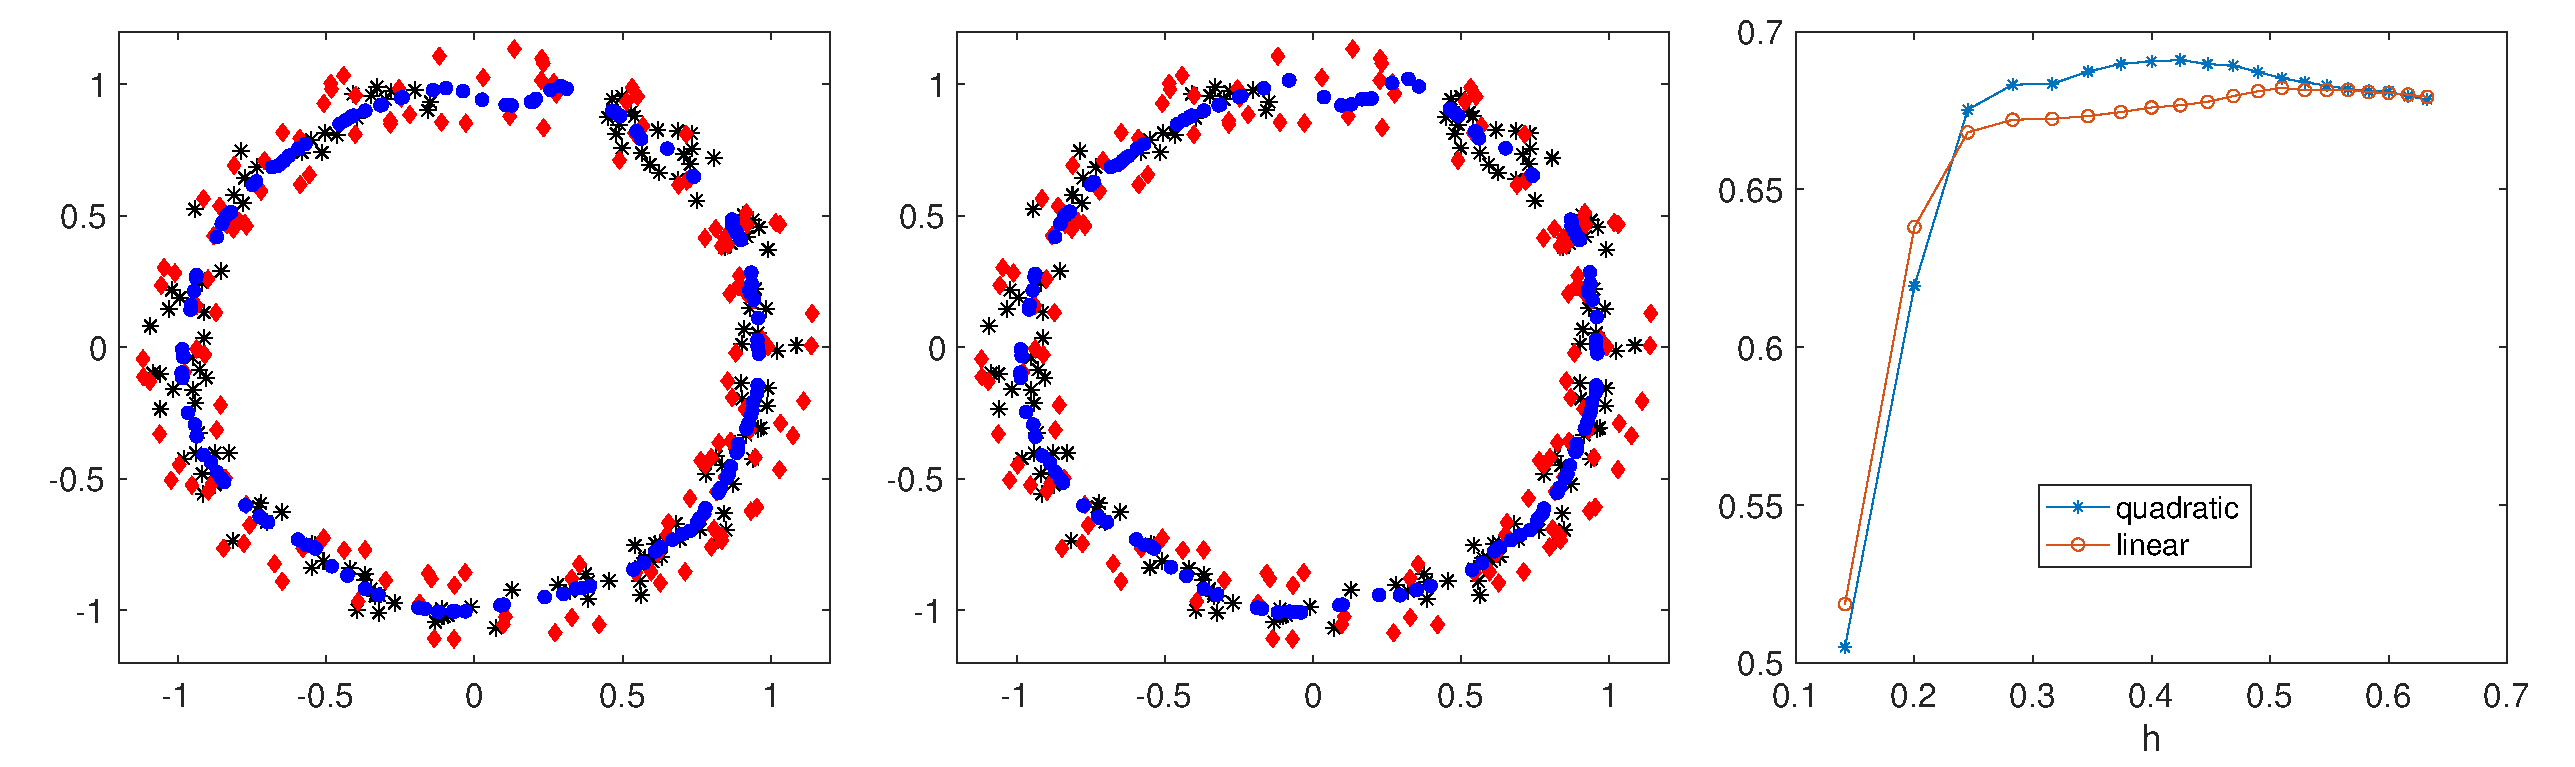
\includegraphics[width=\linewidth]{circle_result.eps} 
     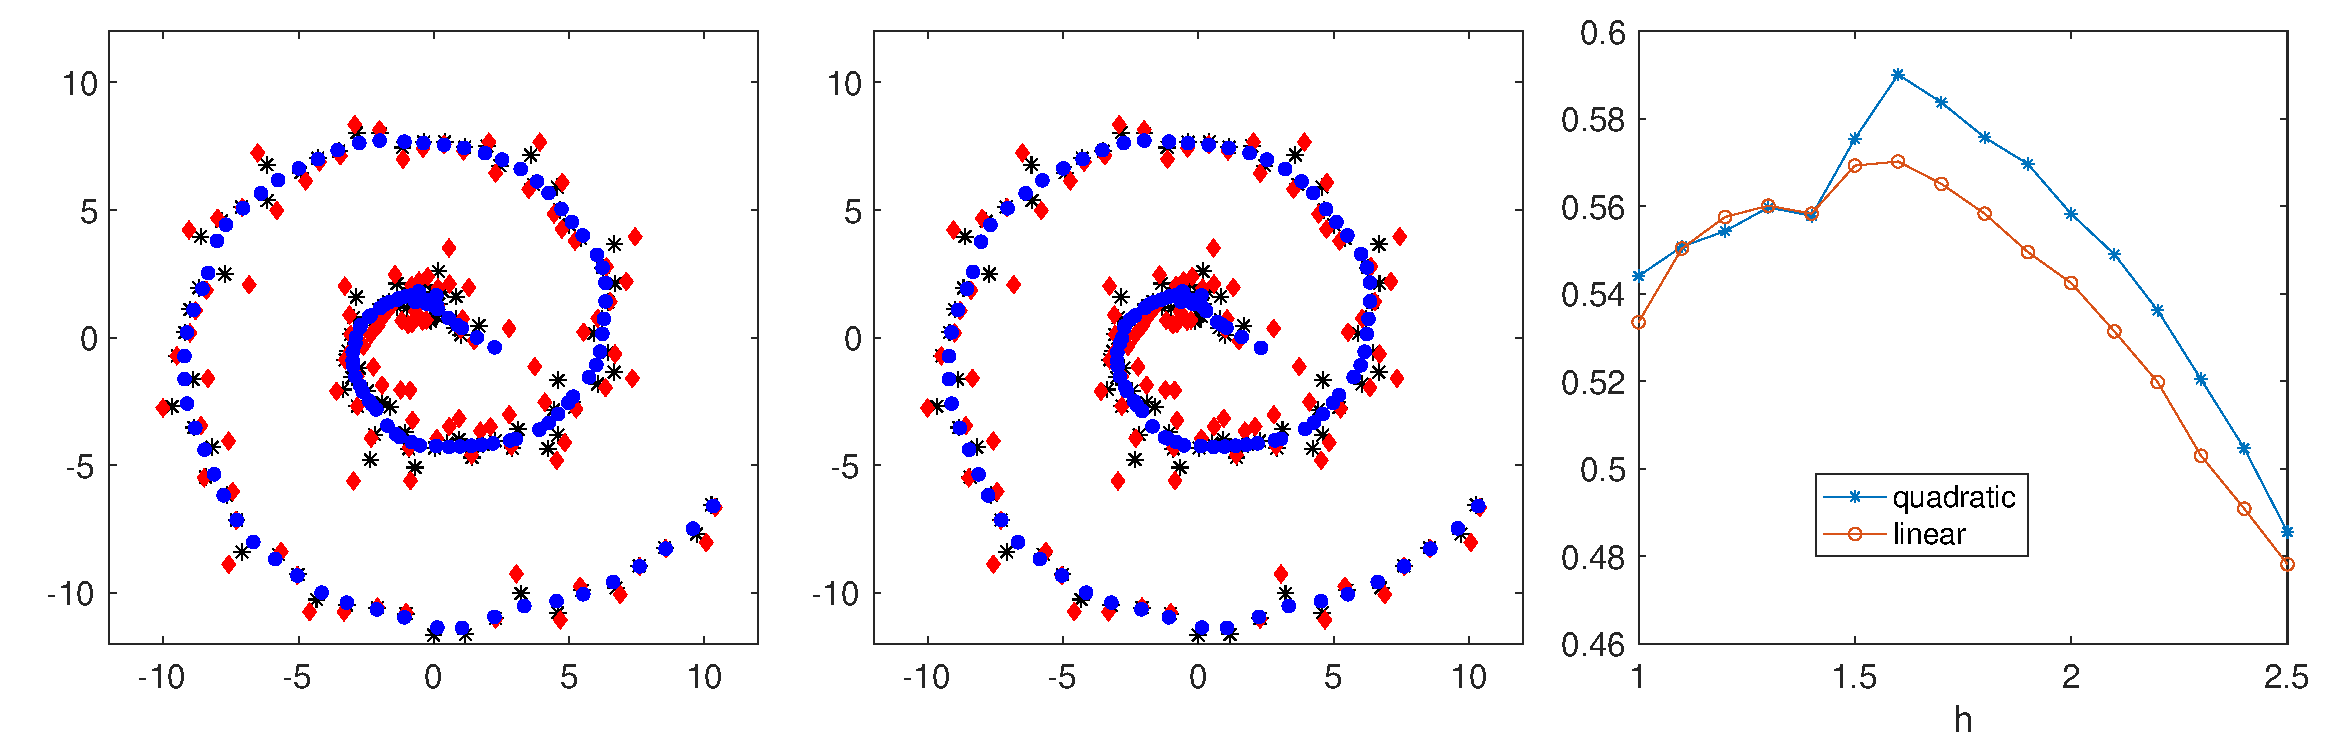
\includegraphics[width=\linewidth]{swiss_roll.eps} 
     %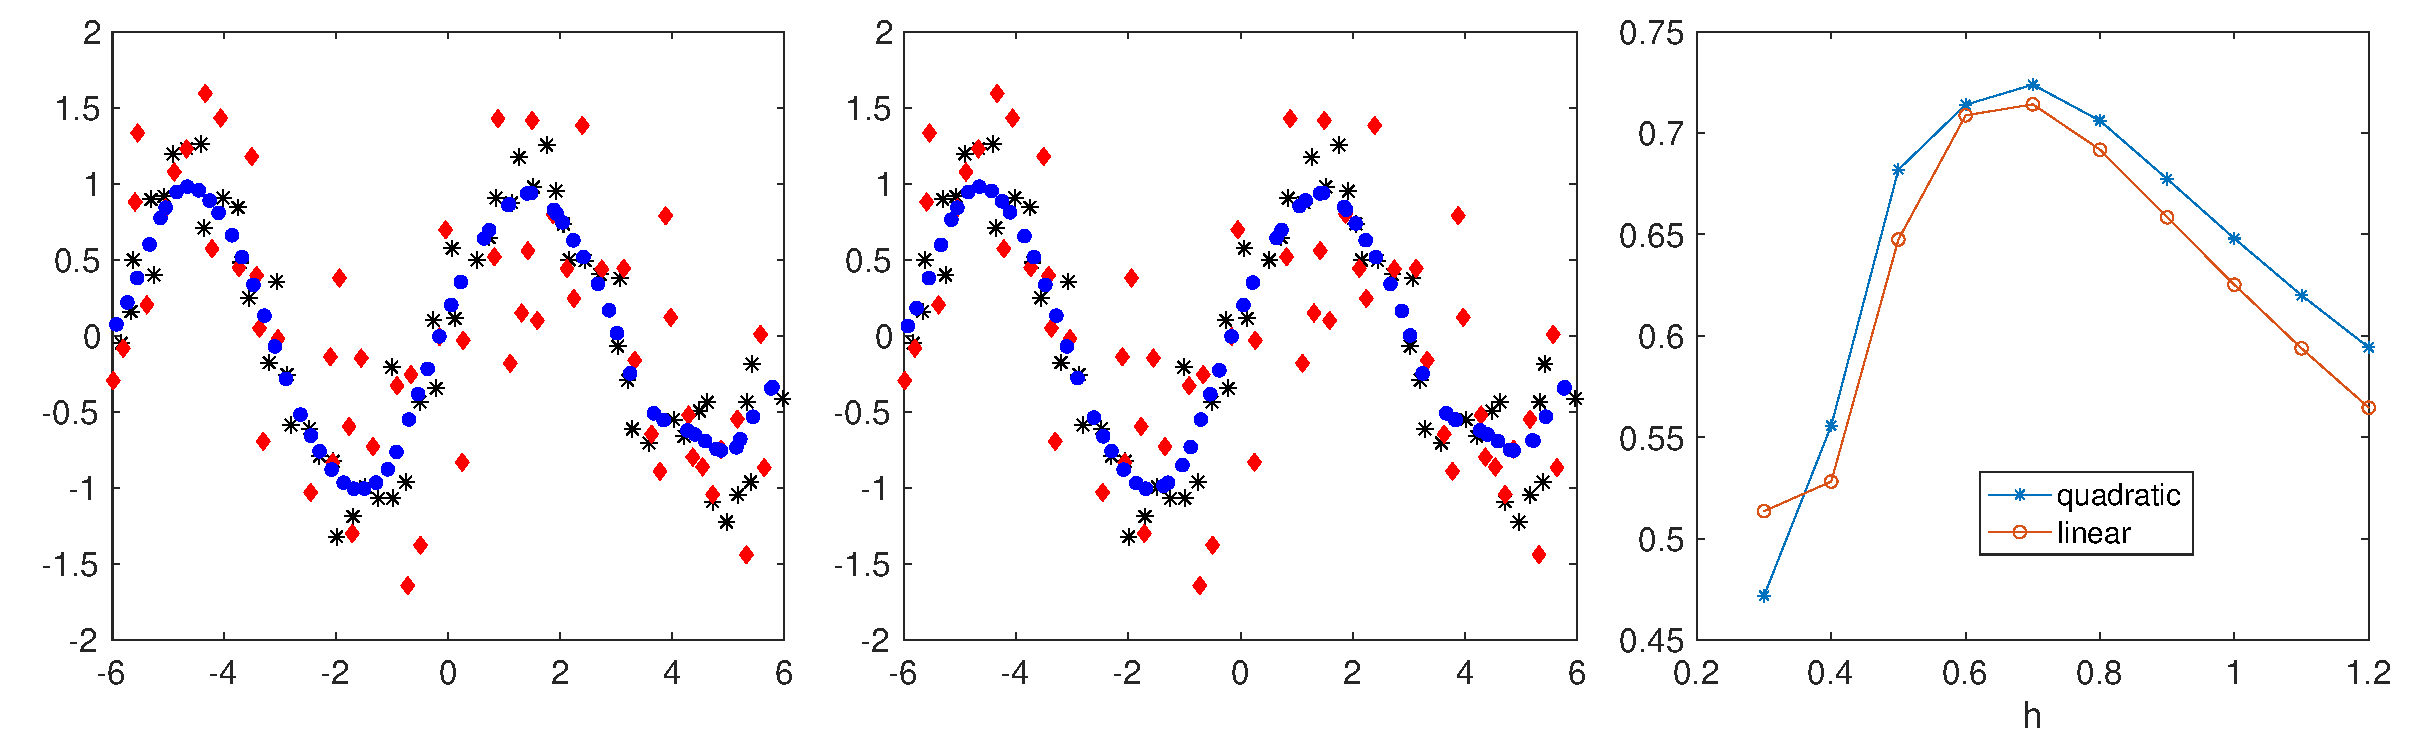
\includegraphics[width=\linewidth]{sin_curve2.eps} 
     \vspace{-0.4cm}
   \caption{Comparison between nonlinear projection and linear projection. Left: nonlinear approach. Right: linear approach}
   \label{fig:sin_curve}
\end{figure}

It is difficult to fit the data drawn from a manifold which is assumed to have varying curvature using a linear model or a tangent plane. Because for $x$ in an area which leads $\kappa(\theta)$ small, the manifold can be approximated by a low-dimensional affine space (a flat plane). However, in a area which has the large curvature $\kappa(\theta)$, such as $\theta=\pi/2$ in our triangle curve case, it is impossible to approximate $y = \sin(\theta)$ by a flat structure. Therefore, it is quit necessary to use a more complicated model to approximate. 

Noting that, our nonlinear second-order fitting function $x_{\cal A}$ is a generalization of the linear function $x_\ell$. When the second order parameter $\cal A$ equal to zero, the derived manifold $\cal M_A$ will degenerate into ${\cal M}_\ell$. By learning $\cal A$, we automatically considering the curvature information hidden in the manifold. Since our nonlinear second-order fitting model $\cal M_A$ is more complicated by having more parameters compared with ${\cal M}_\ell$, we need to use more data to solve our model. Solving the least square problem with too few data will lead to a phenomenon called `overfitting'. When the overfitting phenomenon occurs, the model will not only learn from the true signal of the underlining manifold, but also the noise factors which will distort our model.

In our fitting model, the number of points used is controlled by the bandwidth parameter $h$. Because the kernel weight is decreased fast with the radius, the contribution of the points resides far from our interested area is ignorable. As a result, our model works well with a relatively larger $h$, which can be seen in the rightmost partition of Figure \eqref{fig:sin_curve}. In Figure \eqref{fig:sin_curve}, we randomly samples the black stars `*' as $x_i = \tilde{x}_i+\sigma_1\epsilon_i$ and the red diamonds `$\diamond$' as $x_i = \tilde{x}_i+\sigma_2\epsilon_i$, where $\tilde{x}_i$ is on the underlining $\cal M$ and $\epsilon_i$ is in the normal space of $\cal M$ at $\tilde{x}_i$. In our experimental setting, we have $\sigma_1=0.2$ and $\sigma_2=0.5$ and the length of $\epsilon_i$ obeys the normal distribution of $N(0,1)$. The blue dots `$\circ$' represent the result, which is the projection onto the fitted structure. 

The leftmost figure is the result obtained from the projection onto the nonlinear $\cal M_A$ and the middle figure stands for the result obtained from the projection onto $\cal M_\ell$.
The rightmost figure shows that with the increasing of the bandwidth $h$, the nonlinear projection result has a better performance (under the measurement of $c({\hat{\cal M}})$) in data recovery aspect compared with the linear projection.

%\begin{figure}[t] %  figure placement: here, top, bottom, or page
%   \centering
%   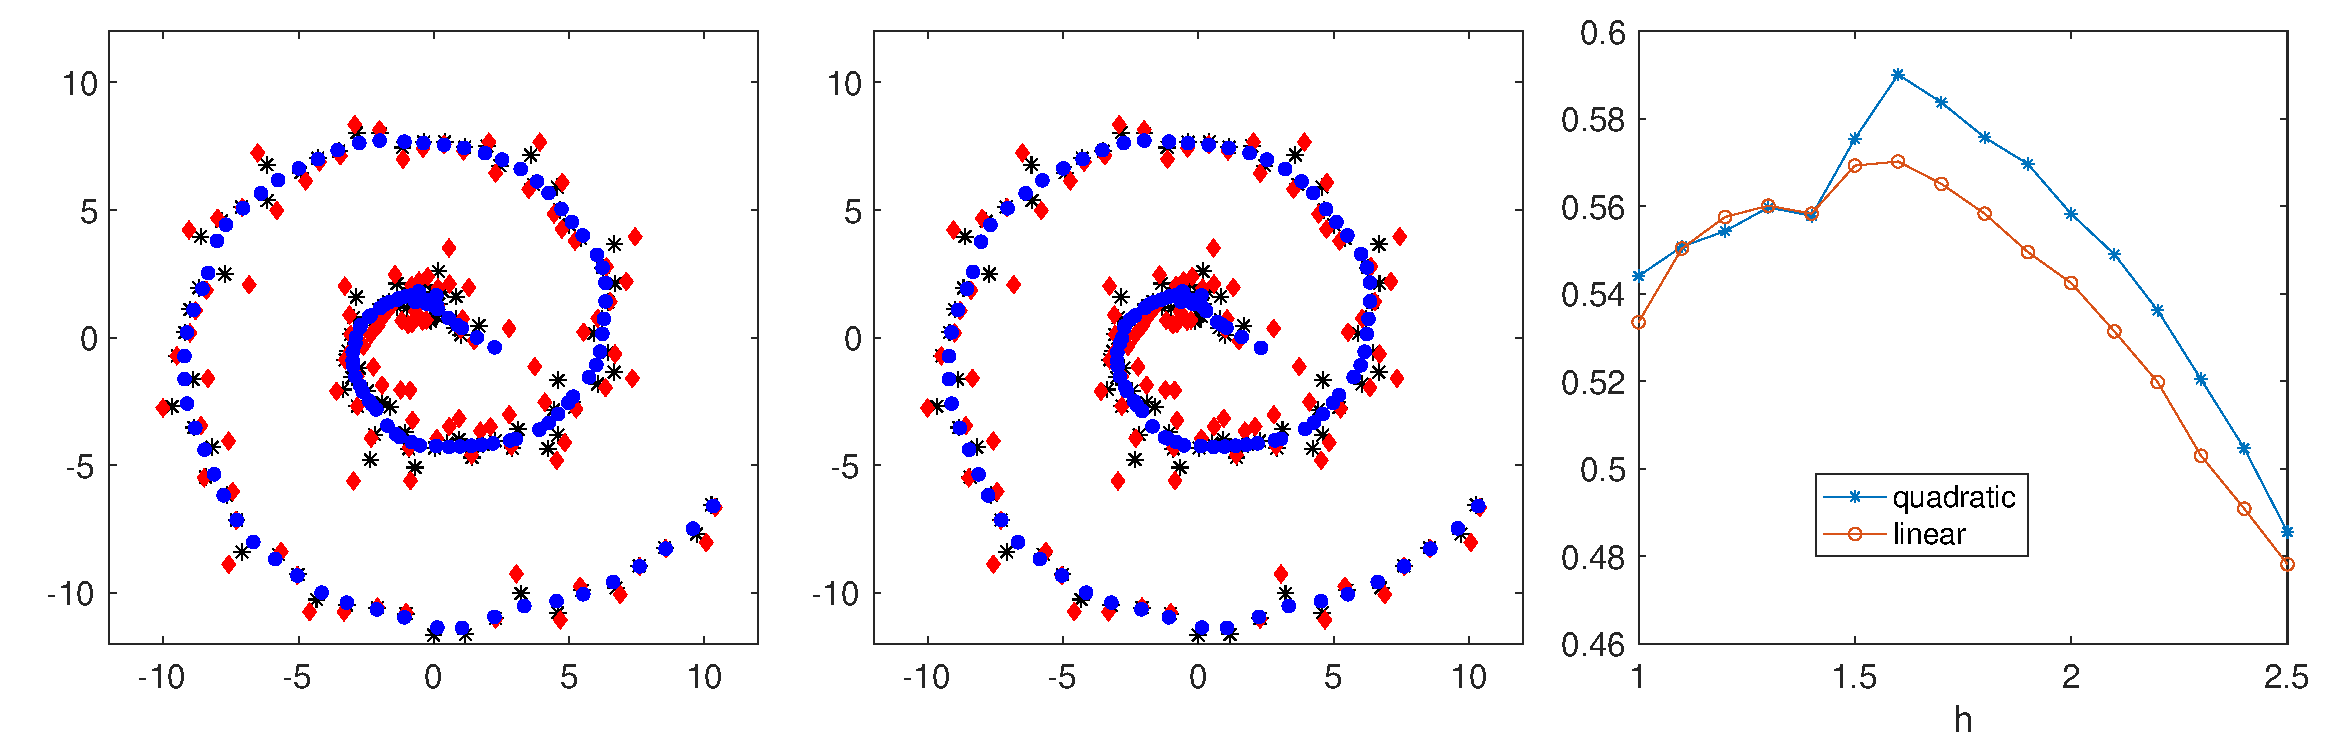
\includegraphics[width=\linewidth]{swiss_roll.eps} 
%   \caption{Comparison between nonlinear projection and linear projection. Left: nonlinear approach. Right: linear approach}
%   \label{fig:sin_curve}
%\end{figure}
\subsection{Real Data}
COIL-20 \cite{COIL-20} is a classical manifold image dataset where the photos are taken by rotating an object with a constant speed. As a consequence, the photos of the same object can be thought drawn from a one-dimensional manifold and disturbed by some noise where the intrinsic variable is the rotated angle. %The images of the same person or object taken under the different angles or illumination can be thought as data drawn from a low-dimensional manifold. %The images can be thought as vector residing in the relatively high-dimensional space, because the dimension is $m*n$ for an image of size $m\times n$. In our algorithm, we need to estimate the local tangent space from the eigen-decomposition. The computational complexity is $O(m^3*n^3)$ for the eigen-decomposition of the covariance matrix of shape $(m*n)\times (m*n)$, which is very expensive.Therefore, if we can apply some methods to reduce the dimension of images by keeping the majority useful information, the computation requirement will be largely reduced.
In order to speed up the algorithm, eigen-face is an applicable dimension reduction method to be applied for images. Denote ${\rm Img}$ as the reshape-operation by transforming a vector of size $m*n$ into a matrix of shape $m\times n$. Therefore, we assume the images are generated as
$
I = {\rm Img} (U_{p}(\tilde{x}+\epsilon_1))+\epsilon_2, \tilde{x}\in \cal M,
$
where $\tilde{x}$ is assumed drawn from a $d$ dimensional manifold. The length of the vector $\tilde{x}$ is $p$, which indicates the dimension of the ambient space is $p$. The columns of $U_p$ span a $p$-dimensional subspace in the $m*n$ dimensional Euclidean space. 
Since the images $\{I_1,...,I_n\}$ of the same object share the same $U_p$, as a result, we can recover $U_p$ from the image set through the eigen-decomposion operation.  Then, from the assumption, we know the $p$ dimensional ambient space which the coordinates 
$
\{v_i = U_p^T {\rm vec}(I_i), i = 1,...,k\},
$
of the images under the basis $U_p$ approximately lies on the $d$ dimensional manifold. Therefore, we just need to recover a $d$ dimensional manifold in the ambient space of dimension $p$.


\begin{figure}[h] %  figure placement: here, top, bottom, or page
   \centering
   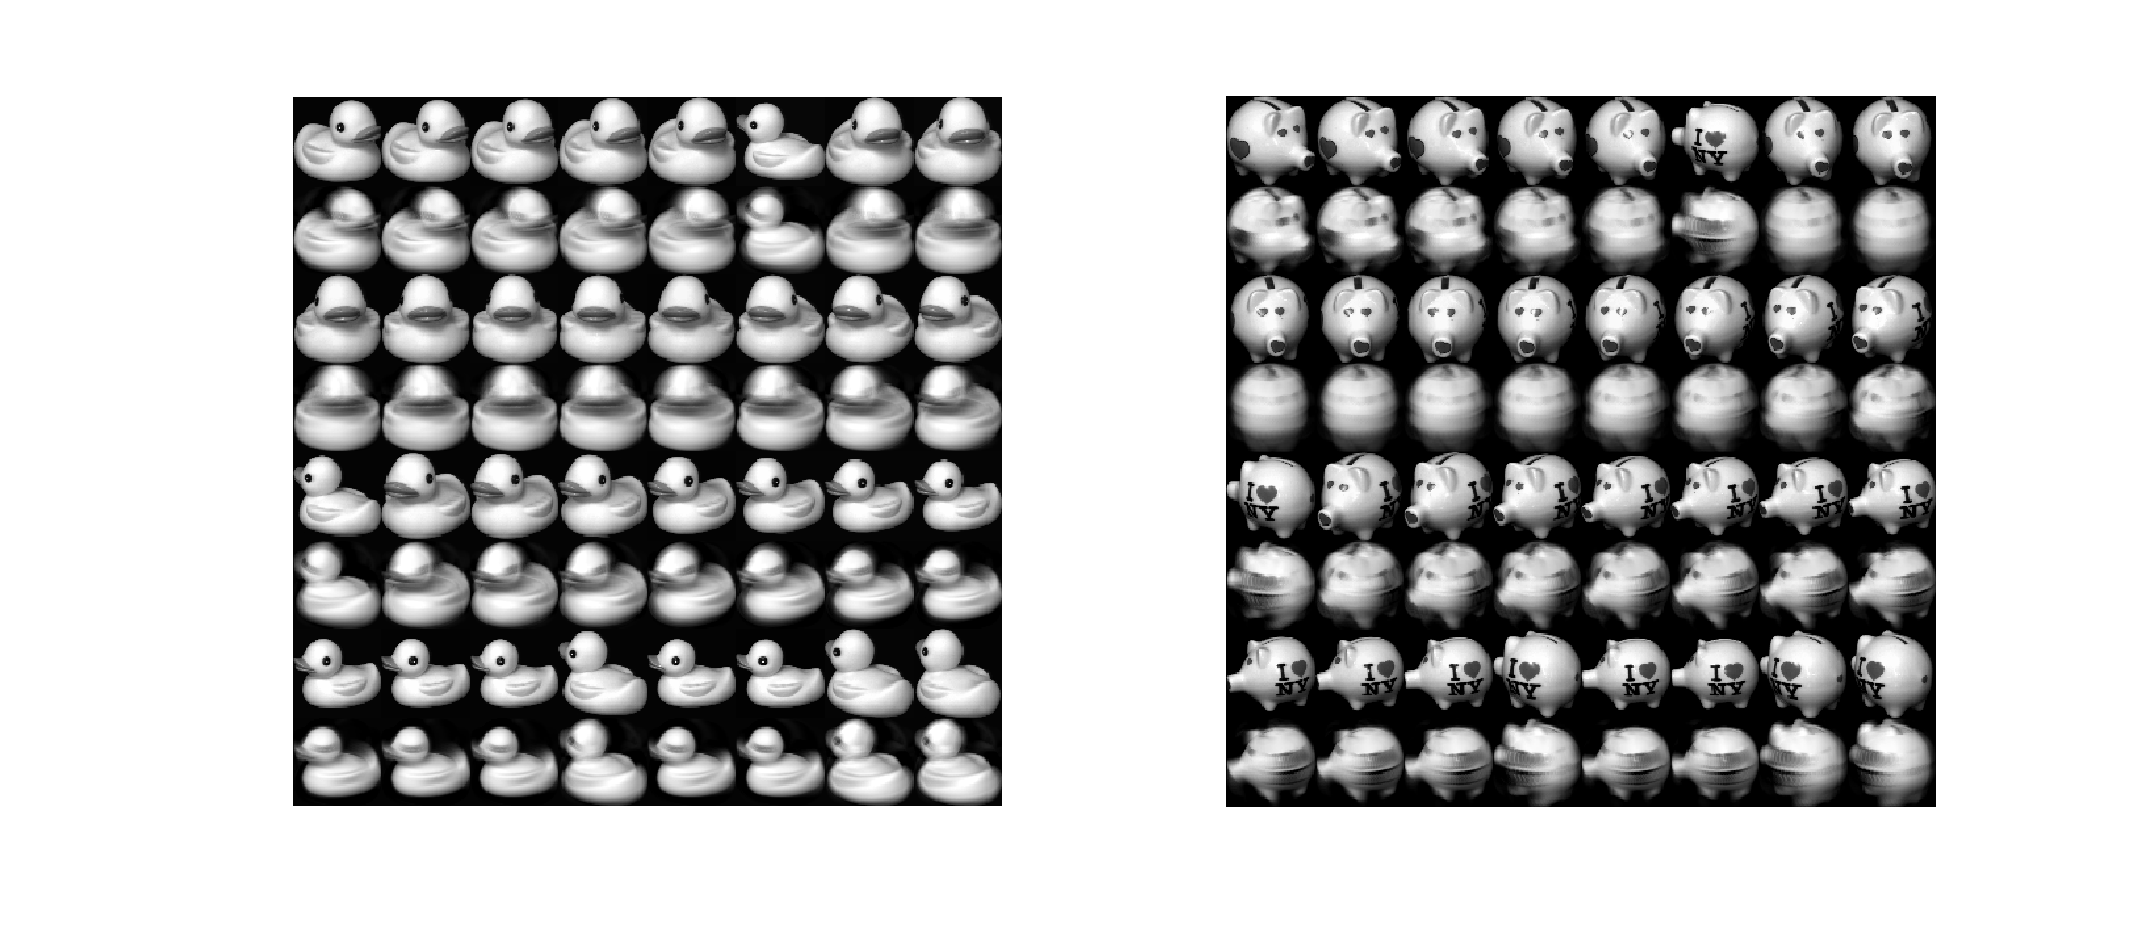
\includegraphics[width=\linewidth]{real.eps} 
   \vspace{-0.4cm}
   \caption{The performance of nonlinear manifold with Coil20 dataset}
   \label{fig:example Coil20}
\end{figure}

With the inputing of the original photo, we could recover a new photo which can be thought as a sample from the underlying smooth manifold. In Figure \ref{fig:example Coil20}, the odd rows are the inputed original photos and the even rows are the output photos of our algorithm. We can see that comparing from the original ones, the sudden change areas of the input photos are smoothed and the rotating trend becomes more apparent than before.


\nocite{langley00}

\bibliography{bibfile}
\bibliographystyle{icml2021}


%%%%%%%%%%%%%%%%%%%%%%%%%%%%%%%%%%%%%%%%%%%%%%%%%%%%%%%%%%%%%%%%%%%%%%%%%%%%%%%
%%%%%%%%%%%%%%%%%%%%%%%%%%%%%%%%%%%%%%%%%%%%%%%%%%%%%%%%%%%%%%%%%%%%%%%%%%%%%%%
% DELETE THIS PART. DO NOT PLACE CONTENT AFTER THE REFERENCES!
%%%%%%%%%%%%%%%%%%%%%%%%%%%%%%%%%%%%%%%%%%%%%%%%%%%%%%%%%%%%%%%%%%%%%%%%%%%%%%%
%%%%%%%%%%%%%%%%%%%%%%%%%%%%%%%%%%%%%%%%%%%%%%%%%%%%%%%%%%%%%%%%%%%%%%%%%%%%%%%
%\appendix
%\section{Do \emph{not} have an appendix here}
%
%\textbf{\emph{Do not put content after the references.}}
%%
%Put anything that you might normally include after the references in a separate
%supplementary file.
%
%We recommend that you build supplementary material in a separate document.
%If you must create one PDF and cut it up, please be careful to use a tool that
%doesn't alter the margins, and that doesn't aggressively rewrite the PDF file.
%pdftk usually works fine. 
%
%\textbf{Please do not use Apple's preview to cut off supplementary material.} In
%previous years it has altered margins, and created headaches at the camera-ready
%stage. 
%%%%%%%%%%%%%%%%%%%%%%%%%%%%%%%%%%%%%%%%%%%%%%%%%%%%%%%%%%%%%%%%%%%%%%%%%%%%%%%
%%%%%%%%%%%%%%%%%%%%%%%%%%%%%%%%%%%%%%%%%%%%%%%%%%%%%%%%%%%%%%%%%%%%%%%%%%%%%%%


\end{document}


% This document was modified from the file originally made available by
% Pat Langley and Andrea Danyluk for ICML-2K. This version was created
% by Iain Murray in 2018, and modified by Alexandre Bouchard in
% 2019 and 2021. Previous contributors include Dan Roy, Lise Getoor and Tobias
% Scheffer, which was slightly modified from the 2010 version by
% Thorsten Joachims & Johannes Fuernkranz, slightly modified from the
% 2009 version by Kiri Wagstaff and Sam Roweis's 2008 version, which is
% slightly modified from Prasad Tadepalli's 2007 version which is a
% lightly changed version of the previous year's version by Andrew
% Moore, which was in turn edited from those of Kristian Kersting and
% Codrina Lauth. Alex Smola contributed to the algorithmic style files.
